%%%%%%%%%%%%%%%%%%%%%%%%%%%%%%%%%%%%%%%%%%%%%%%%%%%%%%%%%%%%%%%%%%%%%%
% Template for a UBC-compliant dissertation
% At the minimum, you will need to change the information found
% after the "Document meta-data"
%
%!TEX TS-program = pdflatex
%!TEX encoding = UTF-8 Unicode

%% The ubcdiss class provides several options:
%%   gpscopy (aka fogscopy)
%%       set parameters to exactly how GPS specifies
%%         * single-sided
%%         * page-numbering starts from title page
%%         * the lists of figures and tables have each entry prefixed
%%           with 'Figure' or 'Table'
%%       This can be tested by `\ifgpscopy ... \else ... \fi'
%%   10pt, 11pt, 12pt
%%       set default font size
%%   oneside, twoside
%%       whether to format for single-sided or double-sided printing
%%   balanced
%%       when double-sided, ensure page content is centred
%%       rather than slightly offset (the default)
%%   singlespacing, onehalfspacing, doublespacing
%%       set default inter-line text spacing; the ubcdiss class
%%       provides \textspacing to revert to this configured spacing
%%   draft
%%       disable more intensive processing, such as including
%%       graphics, etc.
%%

% For submission to GPS
\documentclass[gpscopy,onehalfspacing,11pt]{ubcdiss}

% For your own copies (looks nicer)
% \documentclass[balanced,twoside,11pt]{ubcdiss}

%%%%%%%%%%%%%%%%%%%%%%%%%%%%%%%%%%%%%%%%%%%%%%%%%%%%%%%%%%%%%%%%%%%%%%
%%%%%%%%%%%%%%%%%%%%%%%%%%%%%%%%%%%%%%%%%%%%%%%%%%%%%%%%%%%%%%%%%%%%%%
%%
%% FONTS:
%% 
%% The defaults below configures Times Roman for the serif font,
%% Helvetica for the sans serif font, and Courier for the
%% typewriter-style font.  Configuring fonts can be time
%% consuming; we recommend skipping to END FONTS!
%% 
%% If you're feeling brave, have lots of time, and wish to use one
%% your platform's native fonts, see the commented out bits below for
%% XeTeX/XeLaTeX.  This is not for the faint at heart. 
%% (And shouldn't you be writing? :-)
%%

%% NFSS font specification (New Font Selection Scheme)
\usepackage{times,mathptmx,courier}
\usepackage[scaled=.92]{helvet}
\usepackage{amsmath}
\usepackage{unicode-math}
\usepackage{amssymb}
\usepackage{subcaption}
\usepackage{hyperref}
\usepackage{cleveref}
\usepackage{geometry}

\geometry{
 a4paper,
 left=32mm,
 right=25mm,
 top=25mm,
 bottom=25mm,
}

%% Math or theory people may want to include the handy AMS macros
%\usepackage{amssymb}
%\usepackage{amsmath}
%\usepackage{amsfonts}

%% The pifont package provides access to the elements in the dingbat font.   
%% Use \ding{##} for a particular dingbat (see p7 of psnfss2e.pdf)
%%   Useful:
%%     51,52 different forms of a checkmark
%%     54,55,56 different forms of a cross (saltyre)
%%     172-181 are 1-10 in open circle (serif)
%%     182-191 are 1-10 black circle (serif)
%%     192-201 are 1-10 in open circle (sans serif)
%%     202-211 are 1-10 in black circle (sans serif)
%% \begin{dinglist}{##}\item... or dingautolist (which auto-increments)
%% to create a bullet list with the provided character.
\usepackage{pifont}

%%%%%%%%%%%%%%%%%%%%%%%%%%%%%%%%%%%%%%%%%%%%%%%%%%%%%%%%%%%%%%%%%%%%%%
%% Configure fonts for XeTeX / XeLaTeX using the fontspec package.
%% Be sure to check out the fontspec documentation.
%\usepackage{fontspec,xltxtra,xunicode}	% required
%\defaultfontfeatures{Mapping=tex-text}	% recommended
%% Minion Pro and Myriad Pro are shipped with some versions of
%% Adobe Reader.  Adobe representatives have commented that these
%% fonts can be used outside of Adobe Reader.
%\setromanfont[Numbers=OldStyle]{Minion Pro}
%\setsansfont[Numbers=OldStyle,Scale=MatchLowercase]{Myriad Pro}
%\setmonofont[Scale=MatchLowercase]{Andale Mono}

%% Other alternatives:
%\setromanfont[Mapping=tex-text]{Adobe Caslon}
%\setsansfont[Scale=MatchLowercase]{Gill Sans}
%\setsansfont[Scale=MatchLowercase,Mapping=tex-text]{Futura}
%\setmonofont[Scale=MatchLowercase]{Andale Mono}
%\newfontfamily{\SYM}[Scale=0.9]{Zapf Dingbats}
%% END FONTS
%%%%%%%%%%%%%%%%%%%%%%%%%%%%%%%%%%%%%%%%%%%%%%%%%%%%%%%%%%%%%%%%%%%%%%
%%%%%%%%%%%%%%%%%%%%%%%%%%%%%%%%%%%%%%%%%%%%%%%%%%%%%%%%%%%%%%%%%%%%%%



%%%%%%%%%%%%%%%%%%%%%%%%%%%%%%%%%%%%%%%%%%%%%%%%%%%%%%%%%%%%%%%%%%%%%%
%%%%%%%%%%%%%%%%%%%%%%%%%%%%%%%%%%%%%%%%%%%%%%%%%%%%%%%%%%%%%%%%%%%%%%
%%
%% Recommended packages
%%
\usepackage{checkend}	% better error messages on left-open environments
\usepackage{graphicx}	% for incorporating external images

%% booktabs: provides some special commands for typesetting tables as used
%% in excellent journals.  Ignore the examples in the Lamport book!
\usepackage{booktabs}

%% listings: useful support for including source code listings, with
%% optional special keyword formatting.  The \lstset{} causes
%% the text to be typeset in a smaller sans serif font, with
%% proportional spacing.
\usepackage{listings}
\lstset{basicstyle=\sffamily\scriptsize,showstringspaces=false,fontadjust}

%% The acronym package provides support for defining acronyms, providing
%% their expansion when first used, and building glossaries.  See the
%% example in glossary.tex and the example usage throughout the example
%% document.
%% NOTE: to use \MakeTextLowercase in the \acsfont command below,
%%   we *must* use the `nohyperlinks' option -- it causes errors with
%%   hyperref otherwise.  See Section 5.2 in the ``LaTeX 2e for Class
%%   and Package Writers Guide'' (clsguide.pdf) for details.
\usepackage[printonlyused,nohyperlinks]{acronym}
%% The ubcdiss.cls loads the `textcase' package which provides commands
%% for upper-casing and lower-casing text.  The following causes
%% the acronym package to typeset acronyms in small-caps
%% as recommended by Bringhurst.
\renewcommand{\acsfont}[1]{{\scshape \MakeTextLowercase{#1}}}

%% color: add support for expressing colour models.  Grey can be used
%% to great effect to emphasize other parts of a graphic or text.
%% For an excellent set of examples, see Tufte's "Visual Display of
%% Quantitative Information" or "Envisioning Information".
\usepackage{color}
\definecolor{greytext}{gray}{0.5}

%% comment: provides a new {comment} environment: all text inside the
%% environment is ignored.
%%   \begin{comment} ignored text ... \end{comment}
\usepackage{comment}

%% The natbib package provides more sophisticated citing commands
%% such as \citeauthor{} to provide the author names of a work,
%% \citet{} to produce an author-and-reference citation,
%% \citep{} to produce a parenthetical citation.
%% We use \citeeg{} to provide examples
\usepackage[numbers,sort&compress]{natbib}
\newcommand{\citeeg}[1]{\citep[e.g.,][]{#1}}

%% The titlesec package provides commands to vary how chapter and
%% section titles are typeset.  The following uses more compact
%% spacings above and below the title.  The titleformat that follow
%% ensure chapter/section titles are set in singlespace.
\usepackage[compact]{titlesec}
\titleformat*{\section}{\singlespacing\raggedright\bfseries\Large}
\titleformat*{\subsection}{\singlespacing\raggedright\bfseries\large}
\titleformat*{\subsubsection}{\singlespacing\raggedright\bfseries}
\titleformat*{\paragraph}{\singlespacing\raggedright\itshape}

%% The caption package provides support for varying how table and
%% figure captions are typeset.
\usepackage[format=hang,indention=-1cm,labelfont={bf},margin=1em]{caption}

%% url: for typesetting URLs and smart(er) hyphenation.
%% \url{http://...} 
\usepackage{url}
\urlstyle{sf}	% typeset urls in sans-serif


%%%%%%%%%%%%%%%%%%%%%%%%%%%%%%%%%%%%%%%%%%%%%%%%%%%%%%%%%%%%%%%%%%%%%%
%%%%%%%%%%%%%%%%%%%%%%%%%%%%%%%%%%%%%%%%%%%%%%%%%%%%%%%%%%%%%%%%%%%%%%
%%
%% Possibly useful packages: you may need to explicitly install
%% these from CTAN if they aren't part of your distribution;
%% teTeX seems to ship with a smaller base than MikTeX and MacTeX.
%%
%\usepackage{pdfpages}	% insert pages from other PDF files
%\usepackage{longtable}	% provide tables spanning multiple pages
%\usepackage{chngpage}	% support changing the page widths on demand
%\usepackage{tabularx}	% an enhanced tabular environment

%% enumitem: support pausing and resuming enumerate environments.
%\usepackage{enumitem}

%% rotating: provides two environments, sidewaystable and sidewaysfigure,
%% for typesetting tables and figures in landscape mode.  
%\usepackage{rotating}

%% subfig: provides for including subfigures within a figure,
%% and includes being able to separately reference the subfigures.
%\usepackage{subfig}

%% ragged2e: provides several new new commands \Centering, \RaggedLeft,
%% \RaggedRight and \justifying and new environments Center, FlushLeft,
%% FlushRight and justify, which set ragged text and are easily
%% configurable to allow hyphenation.
%\usepackage{ragged2e}

%% The ulem package provides a \sout{} for striking out text and
%% \xout for crossing out text.  The normalem and normalbf are
%% necessary as the package messes with the emphasis and bold fonts
%% otherwise.
%\usepackage[normalem,normalbf]{ulem}    % for \sout

%%%%%%%%%%%%%%%%%%%%%%%%%%%%%%%%%%%%%%%%%%%%%%%%%%%%%%%%%%%%%%%%%%%%%%
%% HYPERREF:
%% The hyperref package provides for embedding hyperlinks into your
%% document.  By default the table of contents, references, citations,
%% and footnotes are hyperlinked.
%%
%% Hyperref provides a very handy command for doing cross-references:
%% \autoref{}.  This is similar to \ref{} and \pageref{} except that
%% it automagically puts in the *type* of reference.  For example,
%% referencing a figure's label will put the text `Figure 3.4'.
%% And the text will be hyperlinked to the appropriate place in the
%% document.
%%
%% Generally hyperref should appear after most other packages

%% The following puts hyperlinks in very faint grey boxes.
%% The `pagebackref' causes the references in the bibliography to have
%% back-references to the citing page; `backref' puts the citing section
%% number.  See further below for other examples of using hyperref.
%% 2009/12/09: now use `linktocpage' (Jacek Kisynski): GPS now prefers
%%   that the ToC, LoF, LoT place the hyperlink on the page number,
%%   rather than the entry text.
\usepackage[bookmarks,bookmarksnumbered,%
    allbordercolors={0.8 0.8 0.8},%
    pagebackref,linktocpage%
    ]{hyperref}
%% The following change how the the back-references text is typeset in a
%% bibliography when `backref' or `pagebackref' are used
%%
%% Change \nocitations if you'd like some text shown where there
%% are no citations found (e.g., pulled in with \nocite{xxx})
\newcommand{\nocitations}{\relax}
%%\newcommand{\nocitations}{No citations}
%%
%\renewcommand*{\backref}[1]{}% necessary for backref < 1.33
\renewcommand*{\backrefsep}{,~}%
\renewcommand*{\backreftwosep}{,~}% ', and~'
\renewcommand*{\backreflastsep}{,~}% ' and~'
\renewcommand*{\backrefalt}[4]{%
\textcolor{greytext}{\ifcase #1%
\nocitations%
\or
\(\rightarrow\) page #2%
\else
\(\rightarrow\) pages #2%
\fi}}


%% The following uses most defaults, which causes hyperlinks to be
%% surrounded by colourful boxes; the colours are only visible in
%% PDFs and don't show up when printed:
%\usepackage[bookmarks,bookmarksnumbered]{hyperref}

%% The following disables the colourful boxes around hyperlinks.
%\usepackage[bookmarks,bookmarksnumbered,pdfborder={0 0 0}]{hyperref}

%% The following disables all hyperlinking, but still enabled use of
%% \autoref{}
%\usepackage[draft]{hyperref}

%% The following commands causes chapter and section references to
%% uppercase the part name.
\renewcommand{\chapterautorefname}{Chapter}
\renewcommand{\sectionautorefname}{Section}
\renewcommand{\subsectionautorefname}{Section}
\renewcommand{\subsubsectionautorefname}{Section}

%% If you have long page numbers (e.g., roman numbers in the 
%% preliminary pages for page 28 = xxviii), you might need to
%% uncomment the following and tweak the \@pnumwidth length
%% (default: 1.55em).  See the tocloft documentation at
%% http://www.ctan.org/tex-archive/macros/latex/contrib/tocloft/
% \makeatletter
% \renewcommand{\@pnumwidth}{3em}
% \makeatother

%%%%%%%%%%%%%%%%%%%%%%%%%%%%%%%%%%%%%%%%%%%%%%%%%%%%%%%%%%%%%%%%%%%%%%
%%%%%%%%%%%%%%%%%%%%%%%%%%%%%%%%%%%%%%%%%%%%%%%%%%%%%%%%%%%%%%%%%%%%%%
%%
%% Some special settings that controls how text is typeset
%%
% \raggedbottom		% pages don't have to line up nicely on the last line
% \sloppy		% be a bit more relaxed in inter-word spacing
% \clubpenalty=10000	% try harder to avoid orphans
% \widowpenalty=10000	% try harder to avoid widows
% \tolerance=1000

%% And include some of our own useful macros
% This file provides examples of some useful macros for typesetting
% dissertations.  None of the macros defined here are necessary beyond
% for the template documentation, so feel free to change, remove, and add
% your own definitions.
%
% We recommend that you define macros to separate the semantics
% of the things you write from how they are presented.  For example,
% you'll see definitions below for a macro \file{}: by using
% \file{} consistently in the text, we can change how filenames
% are typeset simply by changing the definition of \file{} in
% this file.
% 
%% The following is a directive for TeXShop to indicate the main file
%%!TEX root = diss.tex

\newcommand{\NA}{\textsc{n/a}}	% for "not applicable"
\newcommand{\eg}{e.g.,\ }	% proper form of examples (\eg a, b, c)
\newcommand{\ie}{i.e.,\ }	% proper form for that is (\ie a, b, c)
\newcommand{\etal}{\emph{et al}}

% Some useful macros for typesetting terms.
\newcommand{\file}[1]{\texttt{#1}}
\newcommand{\class}[1]{\texttt{#1}}
\newcommand{\red}[1]{{\color{red}#1}}
\newcommand{\latexpackage}[1]{\href{http://www.ctan.org/macros/latex/contrib/#1}{\texttt{#1}}}
\newcommand{\latexmiscpackage}[1]{\href{http://www.ctan.org/macros/latex/contrib/misc/#1.sty}{\texttt{#1}}}
\newcommand{\env}[1]{\texttt{#1}}
\newcommand{\BibTeX}{Bib\TeX}


% Define a command \doi{} to typeset a digital object identifier (DOI).
% Note: if the following definition raise an error, then you likely
% have an ancient version of url.sty.  Either find a more recent version
% (3.1 or later work fine) and simply copy it into this directory,  or
% comment out the following two lines and uncomment the third.
\DeclareUrlCommand\DOI{}
\newcommand{\doi}[1]{\href{http://dx.doi.org/#1}{\DOI{doi:#1}}}
%\newcommand{\doi}[1]{\href{http://dx.doi.org/#1}{doi:#1}}

% Useful macro to reference an online document with a hyperlink
% as well with the URL explicitly listed in a footnote
% #1: the URL
% #2: the anchoring text
\newcommand{\webref}[2]{\href{#1}{#2}\footnote{\url{#1}}}

% epigraph is a nice environment for typesetting quotations
\makeatletter
\newenvironment{epigraph}{%
	\begin{flushright}
	\begin{minipage}{\columnwidth-0.75in}
	\begin{flushright}
	\@ifundefined{singlespacing}{}{\singlespacing}%
    }{
	\end{flushright}
	\end{minipage}
	\end{flushright}}
\makeatother

% \FIXME{} is a useful macro for noting things needing to be changed.
% The following definition will also output a warning to the console
\newcommand{\FIXME}[1]{\typeout{**FIXME** #1}\textbf{[FIXME: #1]}}

% Math
\def\R{\mathbb{R}}
\def\argmax{\mathop{\rm arg\,max}}
\newcommand{\argmin}[1]{\mathop{\hbox{argmin}}_{#1}}
\newcommand{\mat}[1]{\begin{bmatrix}#1\end{bmatrix}}
\newcommand{\alignStar}[1]{\begin{align*}#1\end{align*}}
\newcommand{\bfpara}[1]{\paragraph{\textbf{#1}}}
\def\half{\frac 1 2}
\def\cond{\; | \;}

% END


%%%%%%%%%%%%%%%%%%%%%%%%%%%%%%%%%%%%%%%%%%%%%%%%%%%%%%%%%%%%%%%%%%%%%%
%%%%%%%%%%%%%%%%%%%%%%%%%%%%%%%%%%%%%%%%%%%%%%%%%%%%%%%%%%%%%%%%%%%%%%
%%
%% Document meta-data: be sure to also change the \hypersetup information
%%

\title{Understanding Reinforcement Learning for Locomotion}
%\subtitle{If you want a subtitle}

\author{Farzad Abdolhosseini}
\previousdegree{Computer Engineering, Sharif University of Technology, 2017}
%\previousdegree{M. Silly Walks, Another University, 1994}

% What is this dissertation for?
\degreetitle{Master of Science}

\institution{The University of British Columbia}
\campus{Vancouver}

\faculty{The Faculty of Science}
\department{Computer Science}
\submissionmonth{August}
\submissionyear{2019}

%%%%% TODOOOO:
% details of your examining committee
\examiningcommittee{Michiel van de Panne, Computer Science}{Supervisor}
\examiningcommittee{Leonid Sigal, Computer Science}{Supervisory Committee Member}
% \examiningcommittee{Nebulous Name, Department}{Supervisory Committee Member}
% \examiningcommittee{Magnus Monolith, Other Department}{Additional Examiner}

% details of your supervisory committee
% \supervisorycommittee{Ira Crater, Materials Engineering}%
%     {Supervisory Committee Member}
% \supervisorycommittee{Adeline Long, \textsc{CEO} of Aerial Machine
%     Transportation, Inc.}{Supervisory Committee Member}

%% hyperref package provides support for embedding meta-data in .PDF
%% files
\hypersetup{
  pdftitle={Change this title!  (DRAFT: \today)},
  pdfauthor={Johnny Canuck},
  pdfkeywords={Your keywords here}
}

%%%%%%%%%%%%%%%%%%%%%%%%%%%%%%%%%%%%%%%%%%%%%%%%%%%%%%%%%%%%%%%%%%%%%%
%%%%%%%%%%%%%%%%%%%%%%%%%%%%%%%%%%%%%%%%%%%%%%%%%%%%%%%%%%%%%%%%%%%%%%
%% 
%% The document content
%%

%% LaTeX's \includeonly commands causes any uses of \include{} to only
%% include files that are in the list.  This is helpful to produce
%% subsets of your thesis (e.g., for committee members who want to see
%% the dissertation chapter by chapter).  It also saves time by 
%% avoiding reprocessing the entire file.
%\includeonly{intro,conclusions}
%\includeonly{discussion}

\begin{document}

%%%%%%%%%%%%%%%%%%%%%%%%%%%%%%%%%%%%%%%%%%%%%%%%%%
%% From Thesis Components: Tradtional Thesis
%% <http://www.grad.ubc.ca/current-students/dissertation-thesis-preparation/order-components>

% Preliminary Pages (numbered in lower case Roman numerals)
%    1. Title page (mandatory)
\maketitle

%    2. Committee page (mandatory): lists supervisory committee and,
%    if applicable, the examining committee
\makecommitteepage

%    3. Abstract (mandatory - maximum 350 words)
%% The following is a directive for TeXShop to indicate the main file
%%!TEX root = diss.tex

\chapter{Abstract}


Deep reinforcement learning offers a flexible approach to learning physics-based locomotion. However, these methods are known to be sample-inefficient and the result usually has poor motion quality without the use of motion capture data. This work investigates two approaches that can make motions more realistic all the while having an equal or higher learning efficiency.

Using characters with high torque limits in simulation can speed up learning, however, this can degrade the motion quality. We will propose a more appropriate way of enforcing torque limits on the simulated character without degrading the performance. Furthermore, able-bodied humans tend to have a fairly symmetric gait. We will explore methods that can incorporate this knowledge into the learning process which highly increase the motion quality.


% This document provides brief instructions for using the \class{ubcdiss}
% class to write a \acs{UBC}-conformant dissertation in \LaTeX.  This
% document is itself written using the \class{ubcdiss} class and is
% intended to serve as an example of writing a dissertation in \LaTeX.
% This document has embedded \acp{URL} and is intended to be viewed
% using a computer-based \ac{PDF} reader.

% Note: Abstracts should generally try to avoid using acronyms.

% Note: at \ac{UBC}, both the \ac{GPS} Ph.D. defence programme and the
% Library's online submission system restricts abstracts to 350
% words.

% Consider placing version information if you circulate multiple drafts
%\vfill
%\begin{center}
%\begin{sf}
%\fbox{Revision: \today}
%\end{sf}
%\end{center}



\cleardoublepage

%    4. Lay Summary (Effective May 2017, mandatory - maximum 150 words)
%% The following is a directive for TeXShop to indicate the main file
%%!TEX root = diss.tex

%% https://www.grad.ubc.ca/current-students/dissertation-thesis-preparation/preliminary-pages
%% 
%% LAY SUMMARY Effective May 2017, all theses and dissertations must
%% include a lay summary.  The lay or public summary explains the key
%% goals and contributions of the research/scholarly work in terms that
%% can be understood by the general public. It must not exceed 150
%% words in length.

\chapter{Lay Summary}



The lay or public summary explains the key goals and contributions of
the research\slash{}scholarly work in terms that can be understood by the
general public. It must not exceed 150 words in length.

\cleardoublepage

%    5. Preface
%% The following is a directive for TeXShop to indicate the main file
%%!TEX root = diss.tex

\chapter{Preface}

\Cref{ch:envparams} is unpublished work done by myself with inputs as well as help with the idea conception from the supervisor, Michiel van de Panne.

\Cref{ch:symmetry} is under review as Farzad Abdolhosseini, Hung Yu Ling, Zhaoming Xie, Xue Bin Peng, Michiel van de Panne. \textit{On Learning Symmetric Locomotion}. Motion, Interaction and Games 2018. The bulk of the work was done by myself and the second author, Hung Yu (Ben) Ling. Zhaoming Xie and Xue Bin (Jason) Peng also contributed by introducing a novel method as well as conducting some of the experiments. The supervisor, Michiel van de Panne, also helped in writing the paper.

\cleardoublepage

%    6. Table of contents (mandatory - list all items in the preliminary pages
%    starting with the abstract, followed by chapter headings and
%    subheadings, bibliographies and appendices)
\tableofcontents
\cleardoublepage	% required by tocloft package

%    7. List of tables (mandatory if thesis has tables)
\listoftables
\cleardoublepage	% required by tocloft package

%    8. List of figures (mandatory if thesis has figures)
\listoffigures
\cleardoublepage	% required by tocloft package

%    9. List of illustrations (mandatory if thesis has illustrations)
%   10. Lists of symbols, abbreviations or other (optional)

%   11. Glossary (optional)
%% The following is a directive for TeXShop to indicate the main file
%%!TEX root = diss.tex

\chapter{Glossary}

% This glossary uses the handy \latexpackage{acroynym} package to automatically
% maintain the glossary.  It uses the package's \texttt{printonlyused}
% option to include only those acronyms explicitly referenced in the
% \LaTeX\ source.

% use \acrodef to define an acronym, but no listing
\acrodef{UI}{user interface}
\acrodef{PG}{Policy Gradients}
\acrodef{RL}{Reinforcement Learning}
\acrodef{VO}{Variational Optimization}
\acrodef{DDPG}{Deep Deterministic Policy Gradients}
\acrodef{SAC}{Soft Actor-Critic}
\acrodef{UBC}{University of British Columbia}

% The acronym environment will typeset only those acronyms that were
% *actually used* in the course of the document
\begin{acronym}[ANOVA]
\acro{ANOVA}[ANOVA]{Analysis of Variance\acroextra{, a set of
  statistical techniques to identify sources of variability between groups}}
\acro{API}{application programming interface}
\acro{CTAN}{\acroextra{The }Common \TeX\ Archive Network}
\acro{DOI}{Document Object Identifier\acroextra{ (see
    \url{http://doi.org})}}
\acro{GPS}[GPS]{Graduate and Postdoctoral Studies}
\acro{PDF}{Portable Document Format}
\acro{RCS}[RCS]{Revision control system\acroextra{, a software
    tool for tracking changes to a set of files}}
\acro{TLX}[TLX]{Task Load Index\acroextra{, an instrument for gauging
  the subjective mental workload experienced by a human in performing
  a task}}
\acro{UML}{Unified Modelling Language\acroextra{, a visual language
    for modelling the structure of software artefacts}}
\acro{URL}{Unique Resource Locator\acroextra{, used to describe a
    means for obtaining some resource on the world wide web}}
\acro{W3C}[W3C]{\acroextra{the }World Wide Web Consortium\acroextra{,
    the standards body for web technologies}}
\acro{XML}{Extensible Markup Language}


\acro{DRL}{Deep reinforcement learning}
\acro{PPO}{proximal policy optimization}
\acro{TRPO}{trust-region policy optimization}
\acro{MDP}{Markov Decision Process}
\acro{TLM}{torque limit multiplier}
\acro{TL}{torque limit}
\acro{FSM}{finite-state machine}


\end{acronym}

% You can also use \newacro{}{} to only define acronyms
% but without explictly creating a glossary
% 
% \newacro{ANOVA}[ANOVA]{Analysis of Variance\acroextra{, a set of
%   statistical techniques to identify sources of variability between groups.}}
% \newacro{API}[API]{application programming interface}
% \newacro{GOMS}[GOMS]{Goals, Operators, Methods, and Selection\acroextra{,
%   a framework for usability analysis.}}
% \newacro{TLX}[TLX]{Task Load Index\acroextra{, an instrument for gauging
%   the subjective mental workload experienced by a human in performing
%   a task.}}
% \newacro{UI}[UI]{user interface}
% \newacro{UML}[UML]{Unified Modelling Language}
% \newacro{W3C}[W3C]{World Wide Web Consortium}
% \newacro{XML}[XML]{Extensible Markup Language}
	% always input, since other macros may rely on it

\textspacing		% begin one-half or double spacing

%   12. Acknowledgements (optional)
%% The following is a directive for TeXShop to indicate the main file
%%!TEX root = diss.tex

\chapter{Acknowledgments}

Thank those people who helped you. 

Don't forget your parents or loved ones.

You may wish to acknowledge your funding sources.


%   13. Dedication (optional)

% Body of Thesis (not all sections may apply)
\mainmatter

\acresetall	% reset all acronyms used so far

%    1. Introduction
%% The following is a directive for TeXShop to indicate the main file
%%!TEX root = diss.tex

\chapter{Introduction}
\label{ch:Introduction}

\begin{epigraph}
    \emph{If I have seen farther it is by standing on the shoulders of
    Giants.} ---~Sir Isaac Newton (1855)
\end{epigraph}

This document provides a quick set of instructions for using the
\class{ubcdiss} class to write a dissertation in \LaTeX. 
Unfortunately this document cannot provide an introduction to using
\LaTeX.  The classic reference for learning \LaTeX\ is
\citeauthor{lamport-1994-ladps}'s
book~\cite{lamport-1994-ladps}.  There are also many freely-available
tutorials online;
\webref{http://www.andy-roberts.net/misc/latex/}{Andy Roberts' online
    \LaTeX\ tutorials}
seems to be excellent.
The source code for this docment, however, is intended to serve as
an example for creating a \LaTeX\ version of your dissertation.

We start by discussing organizational issues, such as splitting
your dissertation into multiple files, in
\autoref{sec:SuggestedThesisOrganization}.
We then cover the ease of managing cross-references in \LaTeX\ in
\autoref{sec:CrossReferences}.
We cover managing and using bibliographies with \BibTeX\ in
\autoref{sec:BibTeX}. 
We briefly describe typesetting attractive tables in
\autoref{sec:TypesettingTables}.
We briefly describe including external figures in
\autoref{sec:Graphics}, and using special characters and symbols
in \autoref{sec:SpecialSymbols}.
As it is often useful to track different versions of your dissertation,
we discuss revision control further in
\autoref{sec:DissertationRevisionControl}. 
We conclude with pointers to additional sources of information in
\autoref{sec:Conclusions}.

%%%%%%%%%%%%%%%%%%%%%%%%%%%%%%%%%%%%%%%%%%%%%%%%%%%%%%%%%%%%%%%%%%%%%%
\section{Suggested Thesis Organization}
\label{sec:SuggestedThesisOrganization}

The \acs{UBC} \acf{GPS} specifies a particular arrangement of the
components forming a thesis.\footnote{See
    \url{http://www.grad.ubc.ca/current-students/dissertation-thesis-preparation/order-components}}
This template reflects that arrangement.

In terms of writing your thesis, the recommended best practice for
organizing large documents in \LaTeX\ is to place each chapter in
a separate file.  These chapters are then included from the main
file through the use of \verb+\include{file}+.  A thesis might
be described as six files such as \file{intro.tex},
\file{relwork.tex}, \file{model.tex}, \file{eval.tex},
\file{discuss.tex}, and \file{concl.tex}.

We also encourage you to use macros for separating how something
will be typeset (\eg bold, or italics) from the meaning of that
something. 
For example, if you look at \file{intro.tex}, you will see repeated
uses of a macro \verb+\file{}+ to indicate file names.
The \verb+\file{}+ macro is defined in the file \file{macros.tex}.
The consistent use of \verb+\file{}+ throughout the text not only
indicates that the argument to the macro represents a file (providing
meaning or semantics), but also allows easily changing how
file names are typeset simply by changing the definition of the
\verb+\file{}+ macro.
\file{macros.tex} contains other useful macros for properly typesetting
things like the proper uses of the latinate \emph{exempli grati\={a}}
and \emph{id est} (\ie \verb+\eg+ and \verb+\ie+), 
web references with a footnoted \acs{URL} (\verb+\webref{url}{text}+),
as well as definitions specific to this documentation
(\verb+\latexpackage{}+).

%%%%%%%%%%%%%%%%%%%%%%%%%%%%%%%%%%%%%%%%%%%%%%%%%%%%%%%%%%%%%%%%%%%%%%
\section{Making Cross-References}
\label{sec:CrossReferences}

\LaTeX\ make managing cross-references easy, and the \latexpackage{hyperref}
package's\ \verb+\autoref{}+ command\footnote{%
    The \latexpackage{hyperref} package is included by default in this
    template.}
makes it easier still. 

A thing to be cross-referenced, such as a section, figure, or equation,
is \emph{labelled} using a unique, user-provided identifier, defined
using the \verb+\label{}+ command.  
The thing is referenced elsewhere using the \verb+\autoref{}+ command.
For example, this section was defined using:
\begin{lstlisting}
    \section{Making Cross-References}
    \label{sec:CrossReferences}
\end{lstlisting}
References to this section are made as follows:
\begin{lstlisting}
    We then cover the ease of managing cross-references in \LaTeX\
    in \autoref{sec:CrossReferences}.
\end{lstlisting}
\verb+\autoref{}+ takes care of determining the \emph{type} of the 
thing being referenced, so the example above is rendered as
\begin{quote}
    We then cover the ease of managing cross-references in \LaTeX\
    in \autoref{sec:CrossReferences}.
\end{quote}

The label is any simple sequence of characters, numbers, digits,
and some punctuation marks such as ``:'' and ``--''; there should
be no spaces.  Try to use a consistent key format: this simplifies
remembering how to make references.  This document uses a prefix
to indicate the type of the thing being referenced, such as \texttt{sec}
for sections, \texttt{fig} for figures, \texttt{tbl} for tables,
and \texttt{eqn} for equations.

For details on defining the text used to describe the type
of \emph{thing}, search \file{diss.tex} and the \latexpackage{hyperref}
documentation for \texttt{autorefname}.


%%%%%%%%%%%%%%%%%%%%%%%%%%%%%%%%%%%%%%%%%%%%%%%%%%%%%%%%%%%%%%%%%%%%%%
\section{Managing Bibliographies with \BibTeX}
\label{sec:BibTeX}

One of the primary benefits of using \LaTeX\ is its companion program,
\BibTeX, for managing bibliographies and citations.  Managing
bibliographies has three parts: (i) describing references,
(ii)~citing references, and (iii)~formatting cited references.

\subsection{Describing References}

\BibTeX\ defines a standard format for recording details about a
reference.  These references are recorded in a file with a
\file{.bib} extension.  \BibTeX\ supports a broad range of
references, such as books, articles, items in a conference proceedings,
chapters, technical reports, manuals, dissertations, and unpublished
manuscripts. 
A reference may include attributes such as the authors,
the title, the page numbers, the \ac{DOI}, or a \ac{URL}.  A reference
can also be augmented with personal attributes, such as a rating,
notes, or keywords.

Each reference must be described by a unique \emph{key}.\footnote{%
    Note that the citation keys are different from the reference
    identifiers as described in \autoref{sec:CrossReferences}.}
A key is a simple sequence of characters, numbers, digits, and some
punctuation marks such as ``:'' and ``--''; there should be no spaces. 
A consistent key format simiplifies remembering how to make references. 
For example:
\begin{quote}
   \fbox{\emph{last-name}}\texttt{-}\fbox{\emph{year}}\texttt{-}\fbox{\emph{contracted-title}}
\end{quote}
where \emph{last-name} represents the last name for the first author,
and \emph{contracted-title} is some meaningful contraction of the
title.  Then \citeauthor{kiczales-1997-aop}'s seminal article on
aspect-oriented programming~\cite{kiczales-1997-aop} (published in
\citeyear{kiczales-1997-aop}) might be given the key
\texttt{kiczales-1997-aop}.

An example of a \BibTeX\ \file{.bib} file is included as
\file{biblio.bib}.  A description of the format a \file{.bib}
file is beyond the scope of this document.  We instead encourage
you to use one of the several reference managers that support the
\BibTeX\ format such as
\webref{http://jabref.sourceforge.net}{JabRef} (multiple platforms) or
\webref{http://bibdesk.sourceforge.net}{BibDesk} (MacOS\,X only). 
These front ends are similar to reference manages such as
EndNote or RefWorks.


\subsection{Citing References}

Having described some references, we then need to cite them.  We
do this using a form of the \verb+\cite+ command.  For example:
\begin{lstlisting}
    \citet{kiczales-1997-aop} present examples of crosscutting 
    from programs written in several languages.
\end{lstlisting}
When processed, the \verb+\citet+ will cause the paper's authors
and a standardized reference to the paper to be inserted in the
document, and will also include a formatted citation for the paper
in the bibliography.  For example:
\begin{quote}
    \citet{kiczales-1997-aop} present examples of crosscutting 
    from programs written in several languages.
\end{quote}
There are several forms of the \verb+\cite+ command (provided
by the \latexpackage{natbib} package), as demonstrated in
\autoref{tbl:natbib:cite}.
Note that the form of the citation (numeric or author-year) depends
on the bibliography style (described in the next section).
The \verb+\citet+ variant is used when the author names form
an object in the sentence, whereas the \verb+\citep+ variant
is used for parenthetic references, more like an end-note.
Use \verb+\nocite+ to include a citation in the bibliography
but without an actual reference.
\nocite{rowling-1997-hpps}
\begin{table}
\caption{Available \texttt{cite} variants; the exact citation style
    depends on whether the bibliography style is numeric or author-year.}
\label{tbl:natbib:cite}
\centering
\begin{tabular}{lp{3.25in}}\toprule
Variant & Result \\
\midrule
% We cheat here to simulate the cite/citep/citet for APA-like styles
\verb+\cite+ & Parenthetical citation (\eg ``\cite{kiczales-1997-aop}''
    or ``(\citeauthor{kiczales-1997-aop} \citeyear{kiczales-1997-aop})'') \\
\verb+\citet+ & Textual citation: includes author (\eg
    ``\citet{kiczales-1997-aop}'' or
    or ``\citeauthor{kiczales-1997-aop} (\citeyear{kiczales-1997-aop})'') \\
\verb+\citet*+ & Textual citation with unabbreviated author list \\
\verb+\citealt+ & Like \verb+\citet+ but without parentheses \\
\verb+\citep+ & Parenthetical citation (\eg ``\cite{kiczales-1997-aop}''
    or ``(\citeauthor{kiczales-1997-aop} \citeyear{kiczales-1997-aop})'') \\
\verb+\citep*+ & Parenthetical citation with unabbreviated author list \\
\verb+\citealp+ & Like \verb+\citep+ but without parentheses \\
\verb+\citeauthor+ & Author only (\eg ``\citeauthor{kiczales-1997-aop}'') \\
\verb+\citeauthor*+ & Unabbreviated authors list 
    (\eg ``\citeauthor*{kiczales-1997-aop}'') \\
\verb+\citeyear+ & Year of citation (\eg ``\citeyear{kiczales-1997-aop}'') \\
\bottomrule
\end{tabular}
\end{table}

\subsection{Formatting Cited References}

\BibTeX\ separates the citing of a reference from how the cited
reference is formatted for a bibliography, specified with the
\verb+\bibliographystyle+ command. 
There are many varieties, such as \texttt{plainnat}, \texttt{abbrvnat},
\texttt{unsrtnat}, and \texttt{vancouver}.
This document was formatted with \texttt{abbrvnat}.
Look through your \TeX\ distribution for \file{.bst} files. 
Note that use of some \file{.bst} files do not emit all the information
necessary to properly use \verb+\citet{}+, \verb+\citep{}+,
\verb+\citeyear{}+, and \verb+\citeauthor{}+.

There are also packages available to place citations on a per-chapter
basis (\latexpackage{bibunits}), as footnotes (\latexpackage{footbib}),
and inline (\latexpackage{bibentry}).
Those who wish to exert maximum control over their bibliography
style should see the amazing \latexpackage{custom-bib} package.

%%%%%%%%%%%%%%%%%%%%%%%%%%%%%%%%%%%%%%%%%%%%%%%%%%%%%%%%%%%%%%%%%%%%%%
\section{Typesetting Tables}
\label{sec:TypesettingTables}

\citet{lamport-1994-ladps} made one grievous mistake
in \LaTeX: his suggested manner for typesetting tables produces
typographic abominations.  These suggestions have unfortunately
been replicated in most \LaTeX\ tutorials.  These
abominations are easily avoided simply by ignoring his examples
illustrating the use of horizontal and vertical rules (specifically
the use of \verb+\hline+ and \verb+|+) and using the
\latexpackage{booktabs} package instead.

The \latexpackage{booktabs} package helps produce tables in the form
used by most professionally-edited journals through the use of
three new types of dividing lines, or \emph{rules}.
% There are times that you don't want to use \autoref{}
Tables~\ref{tbl:natbib:cite} and~\ref{tbl:LaTeX:Symbols} are two
examples of tables typeset with the \latexpackage{booktabs} package.
The \latexpackage{booktabs} package provides three new commands
for producing rules:
\verb+\toprule+ for the rule to appear at the top of the table,
\verb+\midrule+ for the middle rule following the table header,
and \verb+\bottomrule+ for the bottom-most at the end of the table.
These rules differ by their weight (thickness) and the spacing before
and after.
A table is typeset in the following manner:
\begin{lstlisting}
    \begin{table}
    \caption{The caption for the table}
    \label{tbl:label}
    \centering
    \begin{tabular}{cc}
    \toprule
    Header & Elements \\
    \midrule
    Row 1 & Row 1 \\
    Row 2 & Row 2 \\
    % ... and on and on ...
    Row N & Row N \\
    \bottomrule
    \end{tabular}
    \end{table}
\end{lstlisting}
See the \latexpackage{booktabs} documentation for advice in dealing with
special cases, such as subheading rules, introducing extra space
for divisions, and interior rules.

%%%%%%%%%%%%%%%%%%%%%%%%%%%%%%%%%%%%%%%%%%%%%%%%%%%%%%%%%%%%%%%%%%%%%%
\section{Figures, Graphics, and Special Characters}
\label{sec:Graphics}

Most \LaTeX\ beginners find figures to be one of the more challenging
topics.  In \LaTeX, a figure is a \emph{floating element}, to be
placed where it best fits.
The user is not expected to concern him/herself with the placement
of the figure.  The figure should instead be labelled, and where
the figure is used, the text should use \verb+\autoref+ to reference
the figure's label.
\autoref{fig:latex-affirmation} is an example of a figure.
\begin{figure}
    \centering
    % For the sake of this example, we'll just use text
    %\includegraphics[width=3in]{file}
    \Huge{\textsf{\LaTeX\ Rocks!}}
    \caption{Proof of \LaTeX's amazing abilities}
    \label{fig:latex-affirmation}   % label should change
\end{figure}
A figure is generally included as follows:
\begin{lstlisting}
    \begin{figure}
    \centering
    \includegraphics[width=3in]{file}
    \caption{A useful caption}
    \label{fig:fig-label}   % label should change
    \end{figure}
\end{lstlisting}
There are three items of note:
\begin{enumerate}
\item External files are included using the \verb+\includegraphics+
    command.  This command is defined by the \latexpackage{graphicx} package
    and can often natively import graphics from a variety of formats.
    The set of formats supported depends on your \TeX\ command processor.
    Both \texttt{pdflatex} and \texttt{xelatex}, for example, can
    import \textsc{gif}, \textsc{jpg}, and \textsc{pdf}.  The plain
    version of \texttt{latex} only supports \textsc{eps} files.

\item The \verb+\caption+ provides a caption to the figure. 
    This caption is normally listed in the List of Figures; you
    can provide an alternative caption for the LoF by providing
    an optional argument to the \verb+\caption+ like so:
    \begin{lstlisting}
    \caption[nice shortened caption for LoF]{%
	longer detailed caption used for the figure}
    \end{lstlisting}
    \ac{GPS} generally prefers shortened single-line captions
    in the LoF: multiple-line captions are a bit unwieldy.

\item The \verb+\label+ command provides for associating a unique, user-defined,
    and descriptive identifier to the figure.  The figure can be
    can be referenced elsewhere in the text with this identifier
    as described in \autoref{sec:CrossReferences}.
\end{enumerate}
See Keith Reckdahl’s excellent guide for more details,
\webref{http://www.ctan.org/tex-archive/info/epslatex.pdf}{\emph{Using
imported graphics in LaTeX2e}}.

\section{Special Characters and Symbols}
\label{sec:SpecialSymbols}

\LaTeX\ appropriates many common symbols for its own purposes,
with some used for commands (\ie \verb+\{}&%+) and
mathematics (\ie \verb+$^_+), and others are automagically transformed
into typographically-preferred forms (\ie \verb+-`'+) or to
completely different forms (\ie \verb+<>+).
\autoref{tbl:LaTeX:Symbols} presents a list of common symbols and
their corresponding \LaTeX\ commands.  A much more comprehensive list 
of symbols and accented characters is available at:
\url{http://www.ctan.org/tex-archive/info/symbols/comprehensive/}
\begin{table}
\caption{Useful \LaTeX\ symbols}\label{tbl:LaTeX:Symbols}
\centering\begin{tabular}{ccp{0.5cm}cc}\toprule
\LaTeX & Result && \LaTeX & Result \\
\midrule
    \verb+\texttrademark+ & \texttrademark && \verb+\&+ & \& \\
    \verb+\textcopyright+ & \textcopyright && \verb+\{ \}+ & \{ \} \\
    \verb+\textregistered+ & \textregistered && \verb+\%+ & \% \\
    \verb+\textsection+ & \textsection && \verb+\verb!~!+ & \verb!~! \\
    \verb+\textdagger+ & \textdagger && \verb+\$+ & \$ \\
    \verb+\textdaggerdbl+ & \textdaggerdbl && \verb+\^{}+ & \^{} \\
    \verb+\textless+ & \textless && \verb+\_+ & \_ \\
    \verb+\textgreater+ & \textgreater && \\
\bottomrule
\end{tabular}
\end{table}

%%%%%%%%%%%%%%%%%%%%%%%%%%%%%%%%%%%%%%%%%%%%%%%%%%%%%%%%%%%%%%%%%%%%%%
\section{Changing Page Widths and Heights}

The \class{ubcdiss} class is based on the standard \LaTeX\ \class{book}
class~\cite{lamport-1994-ladps} that selects a line-width to carry
approximately 66~characters per line.  This character density is
claimed to have a pleasing appearance and also supports more rapid
reading~\cite{bringhurst-2002-teots}.  I would recommend that you
not change the line-widths!

\subsection{The \texttt{geometry} Package}

Some students are unfortunately saddled with misguided supervisors
or committee members whom believe that documents should have the
narrowest margins possible.  The \latexpackage{geometry} package is
helpful in such cases.  Using this package is as simple as:
\begin{lstlisting}
    \usepackage[margin=1.25in,top=1.25in,bottom=1.25in]{geometry}
\end{lstlisting}
You should check the package's documentation for more complex uses.

\subsection{Changing Page Layout Values By Hand}

There are some miserable students with requirements for page layouts
that vary throughout the document.  Unfortunately the
\latexpackage{geometry} can only be specified once, in the document's
preamble.  Such miserable students must set \LaTeX's layout parameters
by hand:
\begin{lstlisting}
    \setlength{\topmargin}{-.75in}
    \setlength{\headsep}{0.25in}
    \setlength{\headheight}{15pt}
    \setlength{\textheight}{9in}
    \setlength{\footskip}{0.25in}
    \setlength{\footheight}{15pt}

    % The *sidemargin values are relative to 1in; so the following
    % results in a 0.75 inch margin
    \setlength{\oddsidemargin}{-0.25in}
    \setlength{\evensidemargin}{-0.25in}
    \setlength{\textwidth}{7in}       % 1.1in margins (8.5-2*0.75)
\end{lstlisting}
These settings necessarily require assuming a particular page height
and width; in the above, the setting for \verb+\textwidth+ assumes
a \textsc{US} Letter with an 8.5'' width.
The \latexpackage{geometry} package simply uses the page height and
other specified values to derive the other layout values.
The
\href{http://tug.ctan.org/tex-archive/macros/latex/required/tools/layout.pdf}{\texttt{layout}}
package provides a
handy \verb+\layout+ command to show the current page layout
parameters. 


\subsection{Making Temporary Changes to Page Layout}

There are occasions where it becomes necessary to make temporary
changes to the page width, such as to accomodate a larger formula. 
The \latexmiscpackage{chngpage} package provides an \env{adjustwidth}
environment that does just this.  For example:
\begin{lstlisting}
    % Expand left and right margins by 0.75in
    \begin{adjustwidth}{-0.75in}{-0.75in}
    % Must adjust the perceived column width for LaTeX to get with it.
    \addtolength{\columnwidth}{1.5in}
    \[ an extra long math formula \]
    \end{adjustwidth}
\end{lstlisting}


%%%%%%%%%%%%%%%%%%%%%%%%%%%%%%%%%%%%%%%%%%%%%%%%%%%%%%%%%%%%%%%%%%%%%%
\section{Keeping Track of Versions with Revision Control}
\label{sec:DissertationRevisionControl}

Software engineers have used \acf{RCS} to track changes to their
software systems for decades.  These systems record the changes to
the source code along with context as to why the change was required.
These systems also support examining and reverting to particular
revisions from their system's past.

An \ac{RCS} can be used to keep track of changes to things other
than source code, such as your dissertation.  For example, it can
be useful to know exactly which revision of your dissertation was
sent to a particular committee member.  Or to recover an accidentally
deleted file, or a badly modified image.  With a revision control
system, you can tag or annotate the revision of your dissertation
that was sent to your committee, or when you incorporated changes
from your supervisor.

Unfortunately current revision control packages are not yet targetted
to non-developers.  But the Subversion project's
\webref{http://tortoisesvn.net/docs/release/TortoiseSVN_en/}{TortoiseSVN}
has greatly simplified using the Subversion revision control system
for Windows users.  You should consult your local geek.

A simpler alternative strategy is to create a GoogleMail account
and periodically mail yourself zipped copies of your dissertation.

%%%%%%%%%%%%%%%%%%%%%%%%%%%%%%%%%%%%%%%%%%%%%%%%%%%%%%%%%%%%%%%%%%%%%%
\section{Recommended Packages}

The real strength to \LaTeX\ is found in the myriad of free add-on
packages available for handling special formatting requirements.
In this section we list some helpful packages.

\subsection{Typesetting}

\begin{description}
\item[\latexpackage{enumitem}:]
    Supports pausing and resuming enumerate environments.

\item[\latexpackage{ulem}:]
    Provides two new commands for striking out and crossing out text
    (\verb+\sout{text}+ and \verb+\xout{text}+ respectively)
    The package should likely
    be used as follows:
    \begin{verbatim}
    \usepackage[normalem,normalbf]{ulem}
    \end{verbatim}
    to prevent the package from redefining the emphasis and bold fonts.

\item[\latexpackage{chngpage}:]
    Support changing the page widths on demand.

\item[\latexpackage{mhchem}:] 
    Support for typesetting chemical formulae and reaction equations.

\end{description}

Although not a package, the
\webref{http://www.ctan.org/tex-archive/support/latexdiff/}{\texttt{latexdiff}}
command is very useful for creating changebar'd versions of your
dissertation.


\subsection{Figures, Tables, and Document Extracts}

\begin{description}
\item[\latexpackage{pdfpages}:]
    Insert pages from other PDF files.  Allows referencing the extracted
    pages in the list of figures, adding labels to reference the page
    from elsewhere, and add borders to the pages.

\item[\latexpackage{subfig}:]
    Provides for including subfigures within a figure, and includes
    being able to separately reference the subfigures.  This is a
    replacement for the older \texttt{subfigure} environment.

\item[\latexpackage{rotating}:]
    Provides two environments, sidewaystable and sidewaysfigure,
    for typesetting tables and figures in landscape mode.  

\item[\latexpackage{longtable}:]
    Support for long tables that span multiple pages.

\item[\latexpackage{tabularx}:]
    Provides an enhanced tabular environment with auto-sizing columns.

\item[\latexpackage{ragged2e}:]
    Provides several new commands for setting ragged text (\eg forms
    of centered or flushed text) that can be used in tabular
    environments and that support hyphenation.

\end{description}


\subsection{Bibliography Related Packages}

\begin{description}
\item[\latexpackage{bibunits}:]
    Support having per-chapter bibliographies.

\item[\latexpackage{footbib}:]
    Cause cited works to be rendered using footnotes.

\item[\latexpackage{bibentry}:] 
    Support placing the details of a cited work in-line.

\item[\latexpackage{custom-bib}:]
    Generate a custom style for your bibliography.

\end{description}


%%%%%%%%%%%%%%%%%%%%%%%%%%%%%%%%%%%%%%%%%%%%%%%%%%%%%%%%%%%%%%%%%%%%%%
\section{Moving On}
\label{sec:Conclusions}

At this point, you should be ready to go.  Other handy web resources:
\begin{itemize}
\item \webref{http://www.ctan.org}{\ac{CTAN}} is \emph{the} comprehensive
    archive site for all things related to \TeX\ and \LaTeX. 
    Should you have some particular requirement, somebody else is
    almost certainly to have had the same requirement before you,
    and the solution will be found on \ac{CTAN}.  The links to
    various packages in this document are all to \ac{CTAN}.

\item An online
    \webref{http://www.ctan.org/get/info/latex2e-help-texinfo/latex2e.html}{%
	reference to \LaTeX\ commands} provides a handy quick-reference
    to the standard \LaTeX\ commands.

\item The list of 
    \webref{http://www.tex.ac.uk/cgi-bin/texfaq2html?label=interruptlist}{%
	Frequently Asked Questions about \TeX\ and \LaTeX}
    can save you a huge amount of time in finding solutions to
    common problems.

\item The \webref{http://www.tug.org/tetex/tetex-texmfdist/doc/}{te\TeX\
    documentation guide} features a very handy list of the most useful
    packages for \LaTeX\ as found in \ac{CTAN}.

\item The
\webref{http://www.ctan.org/tex-archive/macros/latex/required/graphics/grfguide.pdf}{\texttt{color}}
    package, part of the graphics bundle, provides handy commands
    for changing text and background colours.  Simply changing
    text to various levels of grey can have a very 
    \textcolor{greytext}{dramatic effect}.


\item If you're really keen, you might want to join the
    \webref{http://www.tug.org}{\TeX\ Users Group}.

\end{itemize}

\endinput

Any text after an \endinput is ignored.
You could put scraps here or things in progress.


%    2. Main body
% Generally recommended to put each chapter into a separate file
\chapter{Related Work}
\label{ch:relatedwork}


\section{Motion Symmetry}
Motion symmetry has been a topic of interest for many years in the study of human motion and movement biomechanics. 
Symmetric motions are perceived to be more attractive, e.g., for dance~\cite{danceSymmetry},
and gait symmetry is seen an as a desirable outcome for physiological manipulation~\cite{robinson1987use}.
While symmetry is a common assumption in the study of gait and posture, 
individual gaits often do exhibit asymmetries due to various possible functional causes~\cite{seelet}.
We refer the reader to a past review article~\cite{SADEGHI200034} for insights
into the degree of symmetry of lower limbs movement during able-bodied gait
and the potential influence of limb dominance on the motion symmetry of the lower extremities.
and human gaits~\cite{riskowski}.
It is also not obvious how to best quantify 
the asymmetry of human gaits, and thus specific symmetry metrics have been
proposed~\cite{symmetry_measures,symmetry_phase_portrait}.

The robust control of physics-based character locomotion has been a long-standing challenge
for character animation. We refer the reader to a survey paper for a detailed history~\cite{STAR2012}.  
An early and enduring approach to controller design has been to structure control policies around finite state
machines (FSMs) and feedback rules that use a simplified abstract model or feedback law.  These general
ideas have been applied to human athletics and running~\cite{Hodgins95} and a rich variety of walking
styles~\cite{Yin07,Coros10,LeeYS10}. Many controllers developed for physics-based animation
further use optimization methods to improve controllers developed around an FSM-structure, or use an FSM to 
define phase-dependent objectives for an inverse dynamics optimization to be solved at each time step.
Policy search methods, e.g., stochastic local search or CMA~\cite{Hansen06}, can be used to optimize the 
parameters of the given control structures to achieve a richer variety of motions, e.g.,~\cite{Yin07,Coros11}, and
efficient muscle-driven locomotion~\cite{Wang09}.  
Many of the FSM controllers use hard-coded symmetries, which assign the roles of stance-leg or swing-leg
to the left and right legs, as a function of the FSM state.
It is common in kinematic-based approaches to locomotion, e.g.,~\cite{bruderlin,HoldenPFNN}, 
to also mirror all the available motion data
in order to double the effective size of the data set, and to reflect the often-symmetric nature of human locomotion.
Lastly, trajectory optimization-based methods also commonly assume motion symmetry when convenient, e.g.,~\cite{majkowska2007flipping}.

More recently, locomotion synthesis has attracted significant
attention from the reinforcement learning (RL) community, where the OpenAI Gym tasks have 
become a popular RL benchmark~\cite{ref:OpenAI-Gym}. In this context, symmetry constraints are commonly 
not imposed, and the resulting motions often have noticable asymmetries. 
Further work extends these efforts in a variety of ways, including the traversing challenging terrains~\cite{ref:deepmindParkour}.
More realistic and dynamic motions can be achieved with the help of 
motion-capture clips~\cite{2017-TOG-deepLoco,2018-TOG-deepMimic} and these use
what we refer to as the PHASE symmetry method with the goal of more efficient learning, although with
no robust documented experiments to verify the efficiency gains.
The efficient learning of controllers capable of producing high-quality motion for realistic-strength characters remains
a challenging problem in the absence of motion capture data. Recent work makes
progress on this problem using RL with a combination of energy optimization, learning curriculum, and 
an auxiliary motion symmetry loss~\cite{Yu-SIGGRAPH-2018}, which we shall refer to as the LOSS method.

A recent result investigates how DRL problems can become prone to learning plateaus because
of winner-take-all solution modes~\cite{ray_interf}. These can easily arise in DRL because the distribution of data
for policy learning is directly influenced by the policy itself. Thus in the case of multiple diverging 
decision paths, one of the modes will quickly dominate. The choice of whether to encourage symmetry,
and how to do so, may create an optimization landscape that exhibits similar properties.

\chapter{Background}
\label{ch:background}

\section{Reinforcement Learning}


\label{sec:background_rl}

\ac{RL} emerges from the idea that we humans tend to learn about the world through interaction. We can observe the world around us and act in certain ways in order to achieve our goals and at the same time learn more about the world that we live in. \ac{RL} is a computational approach to learning from interactions with the final goal of maximizing a numerical reward signal \cite{rlbook}.

This approach makes \ac{RL} applicable to a wide variety of applications, but at the same time, this generality proves to be problematic as it yields many challenges. The learner is not told which actions are better or worse and it has to figure everything out itself using a weak reward signal. To make matters worse, the consequences of an action might not be immediately visible to the learner as they might be revealed only after a long duration of time.


\subsection{Markov Decision Process}

The problem formulation in \ac{RL} is based on the concept of a \ac{MDP}. The \ac{MDP} is defined by a tuple $\{\mathcal{S}, \mathcal{A}, P, r, \gamma\}$, where $S \in \mathbb R^n, A \in \mathbb R^m$ are the state space and action space of the problem, the transition function $P: S \times S \times A \to [0, \infty)$ 
is a probability density function, with $P(s_{t+1} \mid s_t, a_t)$ being the probability density of visiting $s_{t+1}$ given that at state $s_t$, the system takes action $a_t$.
The reward function $r: S\times A \to \mathbb R$ gives a scalar reward for each transition of the system. 
$\gamma \in [0, 1]$ is the discount factor. A deterministic \ac{MDP} is a special case where the transition function as well as the initial state distribution are deterministic.

Tasks can be categorized into two categories of \textit{episodic} and \textit{continuing} \cite{rlbook}. Episodic tasks can naturally be divided into subsequences known as \textit{episodes}, such as a single match in sports or one play of a game. Each episode ends after a certain period of time, known as the \textit{time horizon}, has passed or a pre-specified \textit{terminal state} has been reached. In continuing tasks, the task goes on without limit and there is no natural notion of an episode present. Here, we will consider the episodic case with a fixed time horizon $T$; for a more in depth discussion please refer to \cite{rlbook}. The goal of reinforcement learning is to find a parameterized policy $\pi_\theta$, where $\pi_\theta: S \times A \to [0, \infty)$ is the probability density of $a_t$ given $s_t$, that solves the following optimization problem:

\begin{align}
\label{eq:return}
\mathop{\mathrm{max}}_\theta J(\theta) = &\mathbb{E}_{\tau\sim p_\theta}\left[\sum_{t=0}^{T-1}\gamma^t{r({s}_t, {a}_t)} \right].
\end{align}

Here, $\tau = (s_0, a_0, r_0, \dots, s_T)$ is known as a \textit{trajectory} and the probability of encountering a trajectory is computed according to $p_\theta(\tau) = P(s_0) \Pi_{t=0}^{T-1} \pi_\theta(a_t|s_t) P(s_{t+1}|s_t,a_t)$. $\gamma \in [0,1]$ is called the discount factor and controls how much we care about future rewards rather than immediate rewards. The (discounted) sum of the rewards is also known as the \textit{return} of a trajectory:
\begin{align*}
    G(\tau) \doteq \sum_{t=0}^{T-1}\gamma^t{r({s}_t, {a}_t)}.
\end{align*}

Another important categorization of tasks is based on state and action spaces being discrete or continuous. Discrete spaces are generally known to have more well defined solutions, namely tabular algorithms, than the continuous spaces. In this article we will be focusing on tasks where both state and action spaces are continuous.

\section{Policy Gradient Methods}
\label{sec:background_pg}

Over the years many algorithms have been proposed for solving \ac{RL} tasks and each are useful in certain scenarios. This section will explain the \ac{PPO} algorithm which is used in the following chapters. For a discussion of other existing methods please refer to \cite{rl_survey}.

\ac{PPO} belongs to the policy gradient methods class which have been show to work well on continuous tasks. The idea behind the \ac{PG} algorithm is pretty straight-forward. In short, it tries to optimize the average return by (approximately) computing its gradient and taking a gradient ascent step in order to increase it.
% However, doing this naively is not possible. and that is where the algorithm works its magic. Even with such a high-level description, we might be able to guess some of the problems that can arise, such as: how to find the global optima, and are the gradients well-behaved or not. We will get back to these problems soon enough, but let us see how the algorithm works first.

In order to optimize the objective, \ac{PG} directly optimizes the policy $\pi$. One of the underlying assumption of \ac{PG} is that the policy should be stochastic rather than deterministic for this algorithm to work, though this assumption can be relaxed \cite{ddpg}. Furthermore, we assume that this stochastic policy is parametrized by parameters $\theta$ and therefore the algorithm's job is to find the optimal parameters $\theta^*$ that maximize \Cref{eq:return}. Now, in order to maximize the objective, we need to know the gradient $\nabla_\theta J(\theta)$. Since computing this gradient requires knowledge about the dynamics of the \ac{MDP}, \ac{PG} approximates it by using the REINFORCE trick \cite{williams1992simple}:

\begin{align}
    \nabla_\theta J(\theta) &= \nabla_\theta \int G(\tau) p_\theta(\tau) \\
    &= \int G(\tau) \nabla_\theta p_\theta(\tau)\\
    &= \int G(\tau) p_\theta(\tau) \nabla_\theta \log p_\theta(\tau)\\
    &= \mathbb{E}_{\tau \sim p_\theta} \left[ G(\tau) \nabla_\theta \log p_\theta(\tau) \right]
    \label{eq:obj_grad}
\end{align}

We can switch the integral and the gradient operator if the policy is differentiable everywhere. The equality is based on the following identity:

\begin{align*}
    p_\theta(\tau)\nabla_\theta \log p_\theta(\tau) = p_\theta(\tau) \frac{\nabla_\theta p_\theta(\tau)}{p_\theta(\tau)} = \nabla_\theta p_\theta(\tau)
\end{align*}

Next, we can expand $\nabla_\theta \log p_\theta$:

\begin{align}
    \nabla_\theta \log p_\theta &= \nabla_\theta \left[ \log p(s_1) + \sum_{t=1}^T \log \pi_\theta(a_t|s_t) + \log p(s_{t+1} | s_t, a_t) \right]\\
    &= \nabla_\theta \left[ \sum_{t=1}^T \log \pi_\theta(a_t|s_t) \right]\\
    &= \sum_{t=1}^T \nabla_\theta \log \pi_\theta(a_t|s_t)
\end{align}

The extra terms are independent of $\theta$ and therefore they do not contribute to the gradient. Substituting this back into \Cref{eq:obj_grad} we arrive at the following expression. For simplicity the discount factor, $\gamma$, has been set to one:

\begin{align}
    \nabla_\theta J(\theta) &= \mathbb{E}_{\tau \sim p_\theta} \left[ G(\tau) \sum_{t=1}^T \nabla_\theta \log \pi_\theta(a_t|s_t) \right]\\
    &= \mathbb{E}_{\tau \sim p_\theta} \left[ \left( \sum_{t=1}^T r_t \right) \left( \sum_{t=1}^T \nabla_\theta \log \pi_\theta(a_t|s_t) \right) \right]
\end{align}

Using this formulation we can use Monte Carlo sampling \cite{SHAPIRO2003353} to approximately compute the gradient in order to iteratively improve the policy:


\begin{align}
    \nabla_\theta J(\theta) &\approx \frac{1}{N} \sum_{i=1}^{N} \left[ \left( \sum_{t=1}^T r_{i,t} \right) \left( \sum_{t=1}^T \nabla_\theta \log \pi_\theta(a_{i,t}|s_{i,t}) \right) \right]
\end{align}

Where, $\tau_i = (s_{i,1}, a_{i,1}, r_{i,1}, \dots, s_{i,T})$ are sample trajectories from $p_\theta$. With this we arrive at the REINFORCE algorithm \cite{williams1992simple}.

Unfortunately, this is not a good estimator in practice as its variance can be quite high. There are multiple tricks that try to alleviate this problem. The simplest is to increase the number of sampled trajectories $N$, however, this also makes the algorithm less efficient. One observation is that a reward time step $t$ only causally depends on actions that were made until time $t$ and are independent from decisions that are made afterwards. In other words, action $a_t$ can only be responsible for the cost to go from time $t$ forward. With some abuse of notation we can write:
\begin{align}
    \nabla_\theta J(\theta) &\approx \mathbb{E}_{\tau \sim p_\theta} \left[ \sum_{t=1}^T \left( \nabla_\theta \log \pi_\theta(a_t|s_t)  \sum_{t'=t}^T r_t \right) \right]\\
    &= \mathbb{E}_{s_t \sim p_\theta} \left[T \nabla_\theta \log \pi_\theta(a_t|s_t)  \sum_{t'=t}^T r_t \right],
\end{align}
where $s_t$ is any state randomly sampled from a randomly sampled trajectory.

Another trick is to use a learned value function $\hat{V}(s)$ also known as a \textit{critic}. It can be shown that subtracting out a fixed value from the cumulative return in the above formula does not change the value of the expectation. Therefore, if $\hat{V}(s_t)$ is a good estimate of $\sum_{t'=t}^T r_t$ then the following approximator would have lower variance:
\begin{align}
    \nabla_\theta J(\theta) &\approx \mathbb{E}_{s_t \sim p_\theta} \left[T \nabla_\theta \log \pi_\theta(a_t|s_t) \left( \sum_{t'=t}^T r_t - \hat{V}(s_t) \right) \right].
\end{align}

\section{Proximal Policy Optimization (PPO)}

Even with the tricks mentioned above, \ac{PG} is difficult to get working in practice.
This problem is partly attributed to destructive updates, where sometimes during training, a bad update makes the performance suddenly drop rapidly and it takes a long time for the agent to recover.
The \ac{TRPO} algorithm~\cite{trpo} was introduced in order to solve this problem.
The authors claim that the destructive updates happen because the algorithm makes large updates based on an optimistic guess.
Therefore \ac{TRPO} only allows the policy to be updated within a trusted region.
In other words, it is a step-size control mechanism.

Later on, \ac{PPO} was introduced as a faster alternative to \ac{TRPO}. The algorithm slightly changes the \ac{PG} update rule as follows:
\begin{align}
    L_{CLIP} = \mathbb{E}_{s_t \sim p_\theta} \left[ \min \left(r_t(\theta) \hat{A}_t, \text{clip}(r_t(\theta), 1-\epsilon, 1+\epsilon) \hat{A}_t\right) \right],
\end{align}
where the probability ratio is defined as $r_t(\theta) = \frac{\pi_\theta(a_t|s_t)}{\pi_{\theta_{old}}(a_t|s_t)}$ and the advantage is just a shorthand for $\hat{A}_t = \sum_{t'=t}^T r_t - \hat{V}(s_t)$. The hyper-parameter $\epsilon$ controls the step-size and it commonly takes on a value in the range $[0.1,0.2]$. For more information please refer to \cite{ppo}.

Intuitively, by clipping the objective, the flow of gradient is blocked if it tries to push the current policy outside of the interval $[1-\epsilon, 1+\epsilon]$ around the old policy. Therefore, \ac{PPO} has been advertised as enforcing a trust-region on the updates.  Although, the validity of this claim has recently been challenged~\cite{truly_pg}, the fact remains that with the right hyper-parameter setting \ac{PPO} is still one of the best model-free algorithms in practice.

% \chapter{Policy Gradients: A Closer Look}
\label{ch:mixedpg}

Much of the success of modern \ac{RL} is due to model-free \ac{RL} algorithms \red{cite?} \red{is DQN MF or MB?} and a class of algorithms called \ac{PG}. Many people in the community have been criticizing these algorithms including Benjamin Recht \red{cite} most importantly for their sample in-efficiency \red{footnote?}  but the fact remains that \ac{PG} and its variants are among the most widely used algorithms in \ac{RL} today. They have been used to learn in-hand manipulation, highly realistic motion imitation, and highly complex games such as DoTA \red{better examples .. is starcraft PPO too?} \red{cite}.

Their capabilities along with their inefficiency suggests that there is possibly much to be gained by studying the algorithms more carefully in order to better understand their limitations in hopes of improving them. The goal of this chapter is to take a closer look at \ac{PG} and figure out some of the underlying assumptions that usually gets swept up beneath the surface to better understand them and develop better approaches \red{better finish}.

The rest of this chapter is organized as follows. We start with a quick introduction into the framework and how it is usually explained in \Cref{sec:background_pg}. We then discuss how the objective that \ac{PG} uses is different from the original objective in \ac{RL} and in doing so show a relationship between \ac{PG} and \ac{VO} \red{cite} and smoothing methods in \Cref{sec:pg_objective}. In \Cref{sec:pg_conv} we explore a design decision in \ac{PG} and show how we can get to algorithms similar to \ac{SAC} and \ac{DDPG} by choosing the other extreme \red{better wording}. Finally, we propose a method that combines these similar algorithms which we call "Mixed Policy Gradients" in \Cref{sec:pg_mixed}.

\section{What is My Objective Function}
\label{sec:pg_objective}

\section{Where Are My Gradients Coming From}
\label{sec:pg_conv}

\section{Mixed Policy Gradients}
\label{sec:pg_mixed}
\chapter{Torque Limit Considerations}
\label{ch:envparams}

Much effort in reinforcement learning has been spent on finding better or faster algorithms that can solve any \ac{RL} problem in a model-free way, i.e. only through interactions with the environment. However, most success stories, such as TD-Gammon~\cite{tdgammon} and AlphaGo~\cite{alphago}, still required careful engineering. Therefore, we believe that the design of the character and the tasks can be in some cases far more important to achieving superior results than the algorithm itself. In other words, making the problem itself simpler and more compatible with the algorithm used can be more productive than finding new algorithms that claim to solve more difficult problems. In this chapter, we look at the effects of different \ac{TL} settings and we show that a simple torque limit curriculum can help achieve higher rewards and more reliable results.

\section{Introduction}
\label{sec:params_torque}

To measure the strength of a person we can measure the strength of his/her muscles. Similarly, we can measure the strength of a robot by measuring the strength of its motors. To do this, we need to consider each joint separately. A natural measure of strength is the amount of torque that the joint can produce. Furthermore, as ideal robots are consistent and never get tired like humans do, we only need to measure the maximum amount of torque output. Hence, a standard way of representing robot strength is through a \ac{TL} vector. Naturally, a simulated character modelled after a robot needs to have a pre-specified \ac{TL}. The correctness of \ac{TL} is of high importance as it determines the capabilities of the robot. Having a higher or lower \ac{TL} setting, therefore, has serious implications on what the agent can or cannot do and how quickly or more reliably the task can be solved.

Experimenting in a simulator, however, allows us to use torque limits that are much higher or lower than in real life and to investigate their effects. In most applications, lower limits tend to be more desirable. In robotics, using excessive forces can cause damage to the robot as well as its surroundings including any human or animals that may be in its vicinity. Using a low torque limit can be seen as a simple but effective safety mechanism that can alleviate many problems. The consequences of using unrealistic limits in computer graphics may not be as dire, but humans are good at perceiving inconsistent movements performed by human-like characters. An impossibly high jump, pushing a heavy object with one hand, and recovering from a fall by using excessive strength are all immediately recognizable by a human observer. Low limits, on the other hand, are usually not noticeable unless the character or robot fails to accomplish the task at hand, as people rarely ever use maximum strength for day to day tasks.

Consequently, researchers in robotics and computer graphics tend to care about using realistic limits on the characters. On the other hand, the machine learning community is usually less concerned with such details and tends to use characters with excessive \ac{TL}. This has been a source of (informal) complaints from the aforementioned communities.

One common way of compelling the agent to use less force is via an energy consumption cost. This approach is widely used in practice. However, it has two disadvantages. First, the agent can still use excessive force if it so desires. More importantly, the energy consumption can be harmful for training. Therefore, the weight of the energy consumption cost is set low enough that it may be ignored by the agent \cite{Yu-SIGGRAPH-2018}.

We aim to solve both of these problems by using \ac{TL} as hard constraints. As a result, this chapter aims to answer the following questions: how much does the torque limit affect learning and can we make use of this knowledge to find better solutions?

Our results indicate that \ac{TL} settings strongly affect the final solution. Below a certain threshold, the learning algorithm generally fails to find any solution, in a reasonable amount of time, that can solve the task. We demonstrate that this phenomenon is not a consequence of the problem setup but rather a limitation of the optimization procedure by showing the existence of higher-performing solutions with the same setting. Finally, we offer a simple solution to fix this problem by using a curriculum during learning. This helps the agent to learn in a simpler environment and then transfer the learned solution to the more difficult setting.

\section{Environments}

We experiment with a set of existing locomotion environments from  Roboschool~\cite{ref:roboschool}. All characters are simulated using PyBullet~\cite{ref:Pybullet} which is a Python interface for the Bullet3 physics engine. In all of the environments, the task is for the character to walk as far as possible in the forward direction in the allotted time. The reward function also includes terms to encourage the agent to use less energy and stay ``alive'' longer, i.e. to not fall. The observation space in all of these environments consists of root information (root z-coordinate, x and y heading vector, root velocity, roll, and pitch), joint angles, joint angular velocities, and binary foot contact information. The torques are all normalized between $-1$ and $1$.

\bfpara{Walker2D} is a simplified bipedal character whose movements are constrained to a 2D plane. An action is a 6D vector corresponding to torques at the hip, knee, and ankle on both left and right legs. The observation space is 22D and it weighs about 24kg.

\bfpara{Hopper} is a one-legged character constrained to a 2D plane. It is similar to the Walker2D with one leg missing. The action space is 3D where each dimension controls the torque at the hip, knee, and ankle. The observation space is 15D and it weights about 16jg.

\bfpara{HalfCheetah} is a 2D model that closely resembles a quadruped with only a fore and a hind left (no sides). An action is a 6D vector, similar to Walker2D, corresponding to the normalized torques at the thigh, shin, and the foot for each of the fore and hind legs. The observation space is 26D and consists of the same information as Walker2D with the addition of more fine-grained contact information. The character weighs about 38kg.

\bfpara{Ant} is a 3D character that resembles an insect with four legs. It consists of a torso as well as four legs that are each divided into two segments. The action space is 8D and the observation space is 28D containing the same information as Walker2D. Despite being three dimensional, this character is highly stable due to having four legs. The character weighs about 182kg.


\section{Methods}

To experiment with different torque limits we need a way to dynamically modify the limits in each environment. Therefore we slightly modified the aforementioned environments to include a parameter denoted by the \ac{TLM}. \ac{TLM} is a single scalar variable and the torque limits are altogether multiplied by this shared scalar which lets us shrink or expand the limits all at once. It is possible to have a specific multiplier for each joint, however, a single variable is sufficient for the purposes of our work.

We use our implementation of PPO \cite{ppo} for all the experiments\footnote{The source code is available at \url{https://github.com/farzadab/walking-benchmark}}.
The hyper-parameters used can be found in \Cref{sec:envparam_hyperparams}.
Each experiment collected 6 million environment time steps in total and all the experiments were replicated five times each.


% \red{Comment on whether the current limits are realistic or how far they are from reality  +++  mention that Roboschool already has more realistic than MuJoCo.}

% \red{\url{https://www.researchgate.net/figure/Joint-torque-and-power-for-human-hip-knee-and-ankle-in-treadmill-walking-Joint-torques_fig1_272484378}}

% \red{thigh and knee both have a default of 100 Nm, whereas ankle is at 30 Nm}

\section{Results}

In this section, we begin by demonstrating the effect of torque limit on training and then provide a more appropriate way of enforcing this limit.
All plots in this section report the average performance as well as the minimum and maximum across five runs.

\subsection{Torque Limit Baseline Experiments}

To determine how the torque limit can affect the final solution, we run a set of experiments on the Walker2D environment with different values of $TLM$ specified. To rule out the effect of random noise which is an important contributing factor in \ac{DRL} experiments \cite{rl_that_matters} we run each experiment five times with different random seeds and the mean of the data is reported as well as the best and the worst results.

\begin{figure}
    \centering
    \begin{subfigure}[t]{\textwidth}
        \centering
        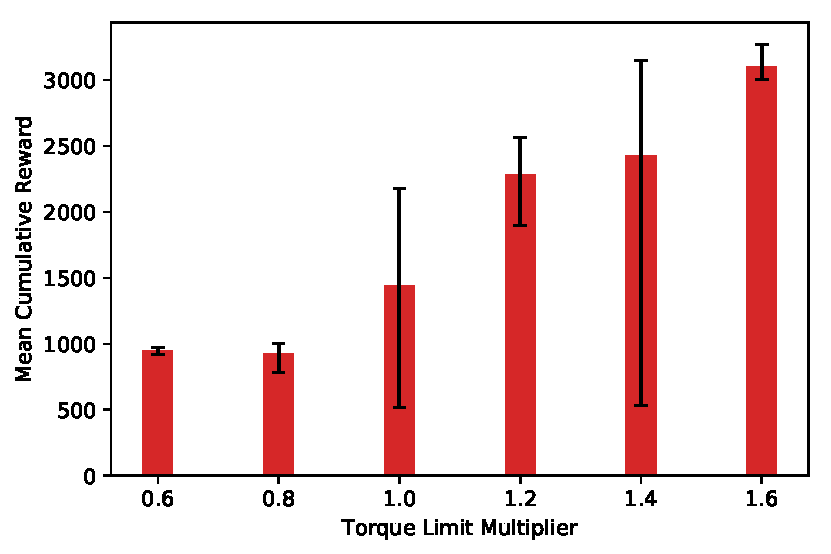
\includegraphics[width=90mm]{img/TorqueLimit_Reward.pdf}
        \caption{Cumulative rewards}
    \end{subfigure}
    \begin{subfigure}[t]{\textwidth}
        \centering
        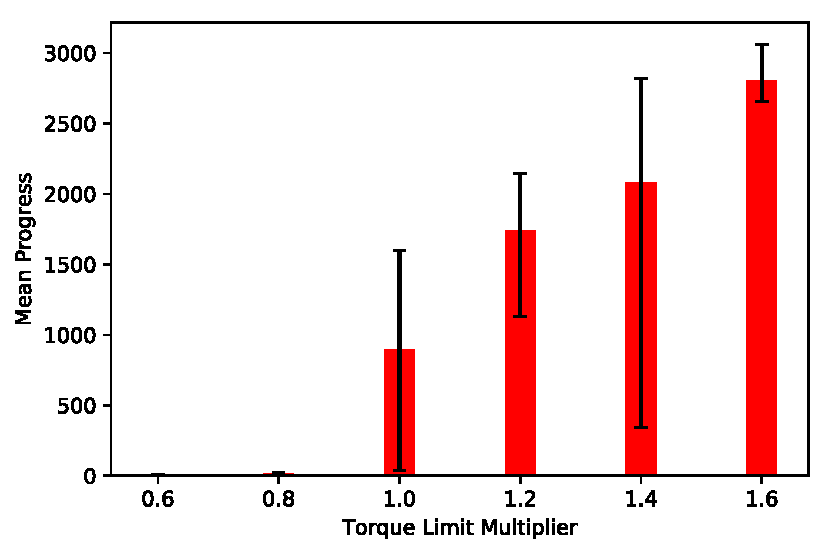
\includegraphics[width=90mm]{img/TorqueLimit_Progress.pdf}
        \caption{Amount of progress in each iteration}
        \label{fig:torque_limit_base_b}
    \end{subfigure}
    \caption{Final performance of the agent with different \ac{TLM} values.}{The error bars reflect the best and the worst performance achieved by the same algorithm over five runs with different random seeds.}
    \label{fig:torque_limit_base}
\end{figure}

The final cumulative return, as well as the amount of progress made at test time, are shown in \Cref{fig:torque_limit_base}. Not surprisingly the agents that had a higher torque limit constraint achieved higher returns. Interestingly, below a certain point (all runs with $TLM \leq 0.8$ as well as some runs with $TLM=1$) the agent failed to make any forward progress. Note that the cumulative return in these cases is still as high as one thousand. This is the result of the agent learning to stand still and avoiding early termination instead of learning to walk.

The results for the default torque limit ($TLM=1$ in the same figure) show us something interesting. First, the variance in the results is high. This is a known problem of reinforcement learning algorithms \cite{rl_that_matters}. More importantly, this hints at the existence of a local optimum where the agent does not learn to move and just avoids early termination by standing still. Even though the results of training with higher torque limits show variations as well, none of them seem to be stuck in this local optima. Lastly, the results seem to indicate that it is not possible to walk with the lower torque limits of 0.6 and 0.8.

\subsection{Torque Limit Curriculum}
If our hypothesis is correct that the agents are getting stuck in a local optimum with lower torque limits, it may be possible to get a better controller simply by using a better initialization. Agents trained with higher torque limits can intuitively provide a good starting point. This leads us to \textit{curriculum learning} \cite{Bengio:2009:CL:1553374.1553380}.

Curriculum learning is motivated by how humans and animals learn and is based on the idea of learning gradually from simple concepts to more difficult ones. In this approach, instead of training on the most difficult version of the problem, the training is divided into multiple stages where the first stage is a simplified version of the problem and task becomes more difficult at each stage until the last stage in which the agent is faced with the original version of the problem.

According to \Cref{fig:torque_limit_base}, tasks with higher torque limits seem to be easier to solve. Therefore, we can define a curriculum where the agent first sees high torque limit environments but gradually the limit is lowered linearly until it matches our final target. To make the training more stationary the training is divided into several levels during which \ac{TLM} stays fixed. The number of these levels is a hyper-parameter denoted by $NLevels$. For most experiments we used $NLevels=10$.

The results of applying the torque limit curriculum can be seen in \Cref{fig:torque_limit_curr}. This method not only achieves higher performance, it also manages to sidestep the local optima as evident in \Cref{fig:torque_limit_curr_b}. As a bonus, this approach seems to be more reliable in most cases as its variance seems to be lower than the baseline approach, except at $TLM=0.6$. In the latter case, the baseline always converges to the local optima which has relatively low variance, however, this is not the desired behaviour.


\begin{figure}
    \centering
    \begin{subfigure}[t]{\textwidth}
        \centering
        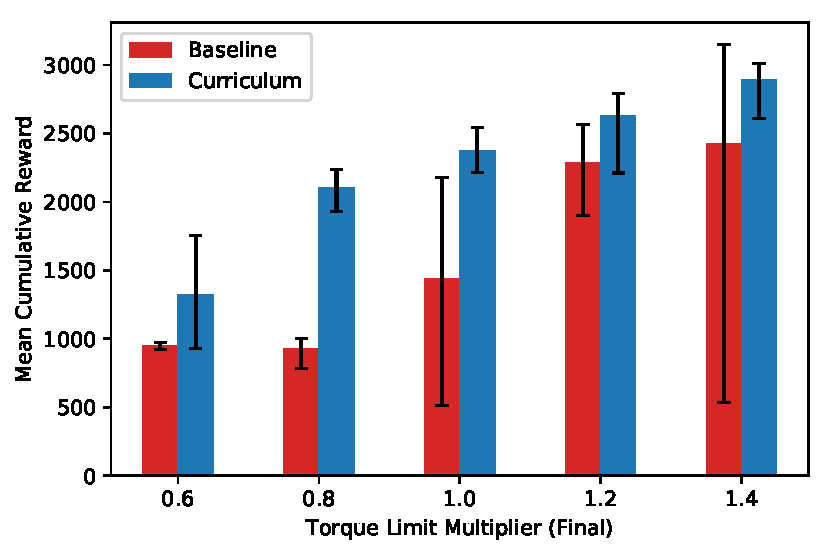
\includegraphics[width=90mm]{img/TorqueLimit_Curr_Reward.pdf}
        \caption{Cumulative rewards}
    \end{subfigure}
    \begin{subfigure}[t]{\textwidth}
        \centering
        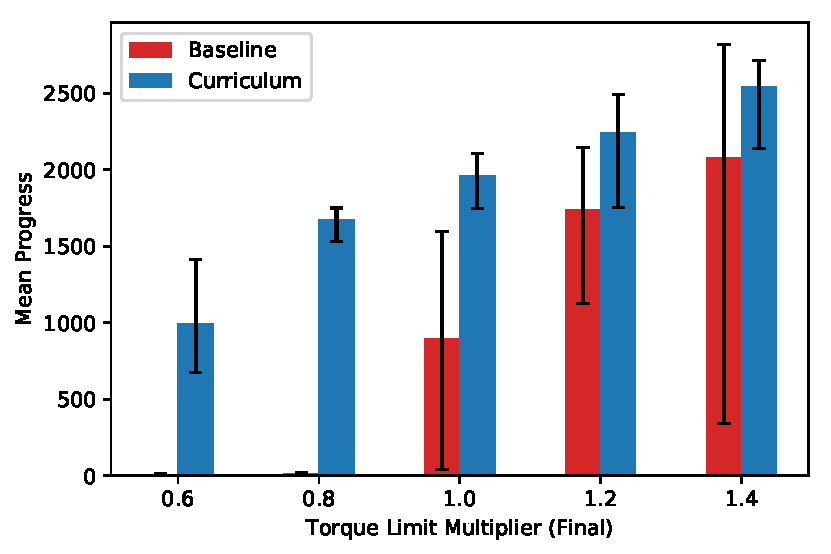
\includegraphics[width=90mm]{img/TorqueLimit_Curr_Progress.pdf}
        \caption{Amount of progress in each iteration}
        \label{fig:torque_limit_curr_b}
    \end{subfigure}
    \caption{The effect of curriculum learning for Walker2D.}{Blue plots show the final performance of the agents which started out with $TLM=1.6$ and the \ac{TLM} was decreased to the target value in ten steps. The red bars are the same as in \Cref{fig:torque_limit_base}.}
    \label{fig:torque_limit_curr}
\end{figure}


\subsection{Ablation and More Environments}

To further validate our approach, we test it on the Half Cheetah, Ant, and Hopper environments as well. As a baseline, we keep \ac{TLM} fixed at the target value.
Also, we compare our results with another curriculum approach that is very similar to our own, namely, an exploration rate curriculum, where the \ac{TLM} is kept fixed the same as in our baseline.
In this approach, the amount of exploration noise is varied at training time by starting at a high value to explore the solution space well and annealing it to a lower value in order to increase the final motion quality.

The results are shown in \Cref{fig:torque_limit_envs}. All experiments used the same hyper-parameters, namely with $NLevels=10$ and the \ac{TLM} going from $1.2$ to $0.6$. The exploration curriculum seems to be helpful to some extent but the \ac{TLM} curriculum works best for all environments, specifically for the Ant.

\begin{figure}
    \centering
    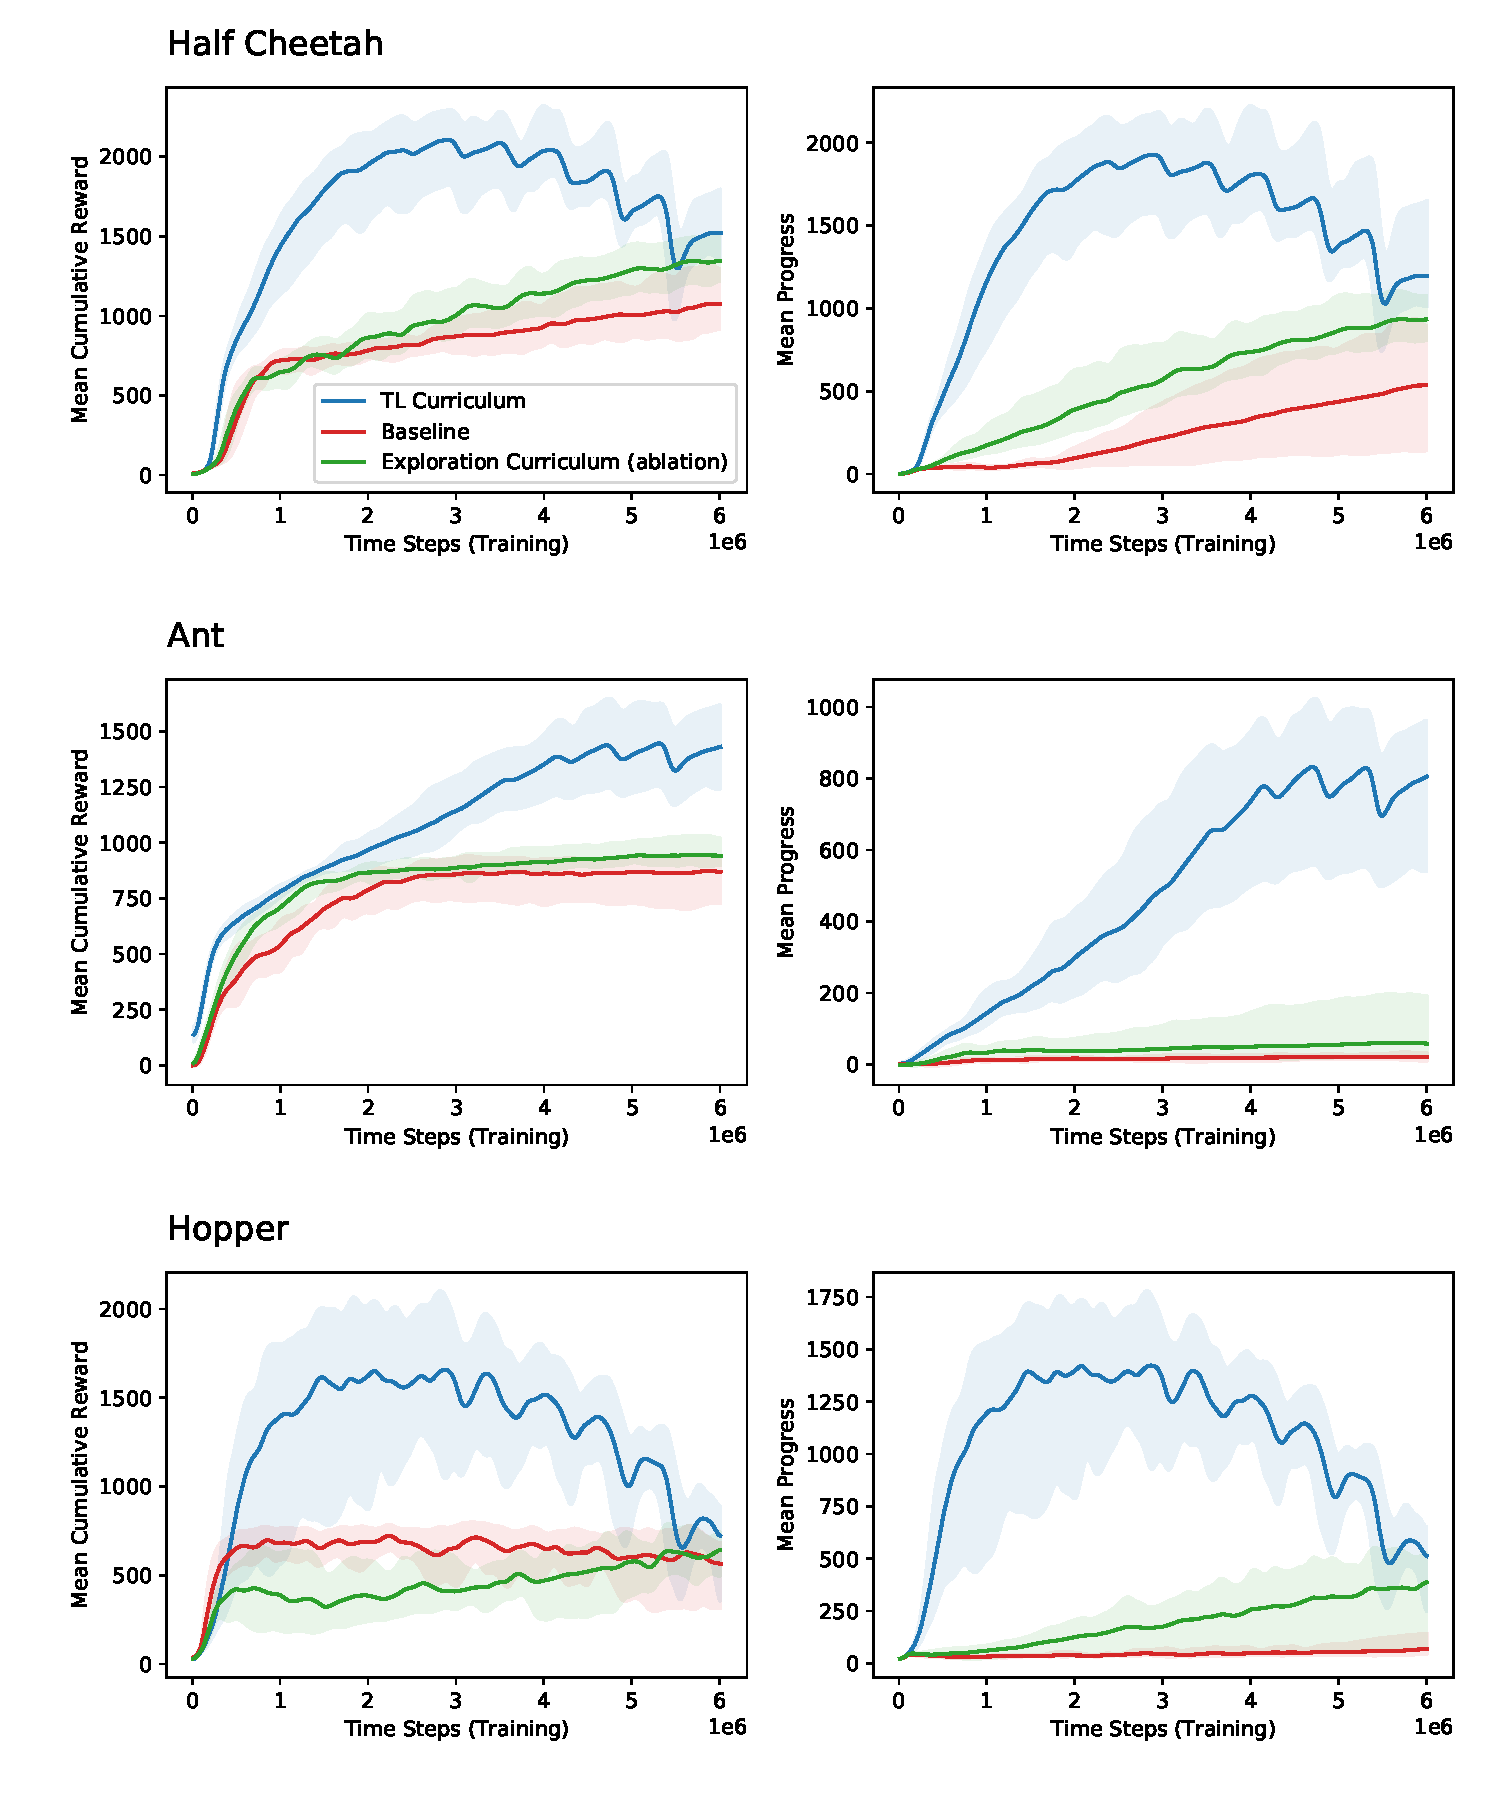
\includegraphics[width=130mm]{img/TorqueLimit_Envs.pdf}
    \caption{Torque limit curriculum results for Half Cheetah, Ant, and Hopper.}{The dips in performance reveal the points in which the value of \ac{TLM} was reduced. The final \ac{TLM} is constant across all methods. The shaded area corresponds to the minimum and the maximum values across five runs.}
    \label{fig:torque_limit_envs}
\end{figure}

\subsection{Curriculum Sensitivity}
\label{subsec:curr_sensitivity}

This curriculum learning technique seems to be useful in the different environments that we tested on, even though the gains vary across domains. However, as with many approaches, this method also includes hyper-parameters that need to be chosen by the user. We can assume that the target torque limits are a given, but the starting limits are not fixed. Furthermore, the optimal value for the \textit{NLevels} hyper-parameter is also unknown. An important question to ask is: how sensitive is this method to the hyper-parameters. Therefore, we designed two experiments to answer this question.

First, we look at the starting \ac{TLM}. We assume that the final \ac{TLM} of $0.6$ is fixed and we can vary the starting \ac{TLM} value. The results of the experiment on the Walker2D environment can be seen in \Cref{fig:torque_limit_hp_tlm}. Surprisingly, all initial values seem to work relatively well. Specifically, by comparing the results for $TLM=0.8$ with \Cref{fig:torque_limit_base_b}, we see that the final performance has increased instead of decreasing even though the final $TLM$ has decreased. This might simply be due to randomness, but it is also possible that the sudden changes in curriculum training let the agent escape local optima regions more easily. More importantly, the results seem to indicate that the method is not sensitive to this hyper-parameter as long as the initial \ac{TLM} value is high enough to stumble upon a good solution.

\begin{figure}
    \centering
    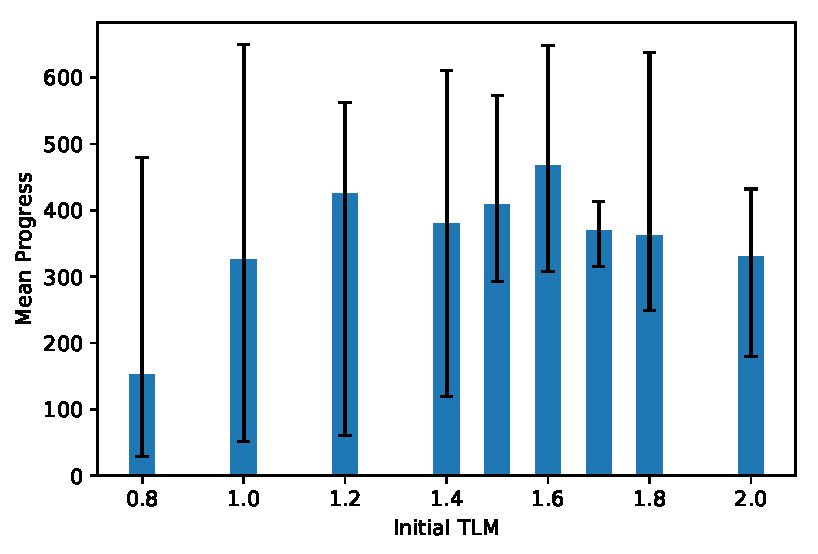
\includegraphics[width=90mm]{img/TorqueLimit_Curr_TLM.pdf}
    \caption{Curriculum sensitivity to initial \ac{TLM} value.}{All experiments with $TLM > 1.2$ have an acceptable performance both in terms of the average as well as the worse performance.}
    \label{fig:torque_limit_hp_tlm}
\end{figure}

Next, we look at the number of curriculum steps required, while keeping the total number of simulation steps fixed. A low number means an abrupt change but a high number would mean changing slowly but frequently. Both approaches have their merits. Changing slowly means the previous solution will still work under the new conditions, but it also means that there might not be enough time to get adjusted to the new situation before the next change. Abrupt changes can also be useful for getting out of a local solution. Again, we run a similar experiment as before on the Walker2D environment with the \ac{TLM} going from $1.6$ to $0.6$ with different number of steps. The results are provided in \Cref{fig:torque_limit_hp_steps}.

\begin{figure}
    \centering
    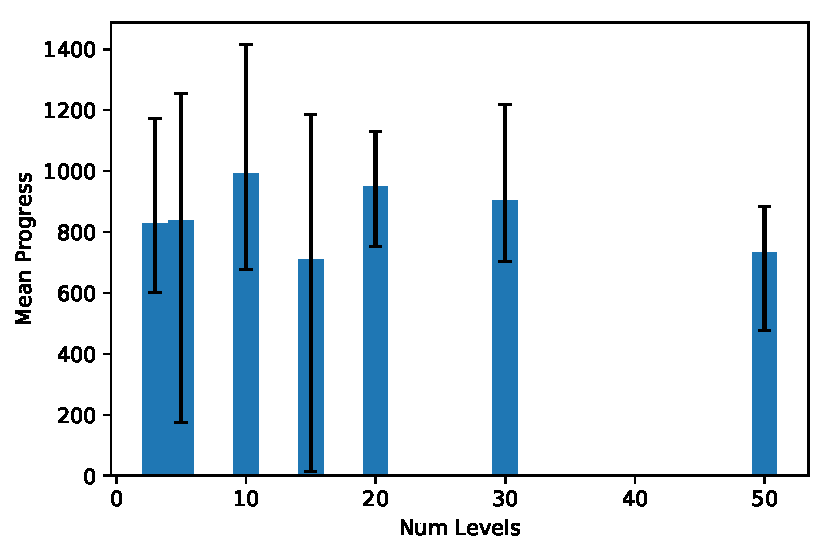
\includegraphics[width=90mm]{img/TorqueLimit_Curr_Steps.pdf}
    \caption{Curriculum sensitivity to the number of steps.}
    \label{fig:torque_limit_hp_steps}
\end{figure}

The results in both cases show some variability, which is to be expected, but there is no clear winner or a general trend to be pointed out. This is reassuring, as it shows that the method is not sensitive to small hyper-parameter changes. This makes the method more easily applicable to different settings.



\section{Conclusions}
In this chapter, we showed that the construction and the details of the locomotion environment are important, and the best design for learning need not be the most realistic one. Here, we looked at the effects of torque limits on learning. Torque limits describe how strong the character is and indirectly decides which movements are possible and which ones are not. The robotics and computer graphics communities tend to specify torque limits based on real-life robots and animals, but the machine learning community is less concerned with such details.

The torque limit setting is indeed important, as evident by the decrease in the final performance achieved in different settings. Furthermore, we show that this setting is specifically important in the context of reinforcement learning since with more restrictive configurations the learner tends to get stuck in local optima regions increasingly often. Therefore doing the initial training with higher torque limits is useful for sidestepping local optima and the resulting policy is perhaps more robust as a result of experiencing slightly different versions of the same environment.


\chapter{Symmetry Considerations}
\label{ch:symmetry}



One obvious path towards faster-and-better learning relies on exploiting the motion symmetry
that is a common attribute of human and animal locomotion;
gait symmetry is an indicator of healthy outcomes in 
physiotherapy~\citep{robinson1987use, riskowski}.
Relatedly, while asymmetric gaits are often associated 
with physical injuries and neural impairments such as stroke.  
A symmetry constraint or symmetry-favouring bias thus offers a readily available and convenient 
path towards faster learning and more realistic outcomes. 
It is also largely orthogonal to most other efficiency improvements.

Naively, exploiting symmetry might be expected to yield a $2\times$ learning speedup, and may help to avoid
some of the undesired asymmetric local minima that \ac{DRL} is prone to exploit.  On the other hand,
it could also be the case that asymmetric policies and motions serve a useful role as an intermediate path 
towards finding eventual optimal symmetric motions, and therefore
hard symmetry constraints may be problematic.
Another important subtlety is that while a symmetric policy helps achieve symmetric motions,
it does not guarantee a symmetric outcome.
For example, a quadruped gallop and a biped lope are asymmetric gait cycles, 
as each gait cycle begins with a leading left or right foot, while the underlying 
policy can still be fully symmetric.

What is the best way to integrate a symmetry bias or other forms of symmetry enforcement into the learning process?
How much benefit does it offer in terms of learning speed and learning outcomes?
What are other considerations for symmetry-informed methods?
The principal contribution of our work is an in-depth analysis of four different methods
of incorporating symmetry into the learning process:
\begin{description}
\item [DUP]  Duplicating tuples with their symmetric counterparts.
\item [LOSS] Adding a symmetry auxiliary loss.
\item [PHASE] Motion phase mirroring.
\item [NET]  Enforcing symmetry in the network itself.
\end{description}
Two of these methods are new (DUP, NET) and two are already present in existing literature (LOSS, PHASE), 
albeit without a systematic evaluation of all the issues around symmetry enforcement. 
The methods incorporate knowledge of symmetry into the policy structure (NET), 
the learning data (DUP, PHASE), or via the learning loss (LOSS). 
We also believe that the results are of more general interest because they 
illustrate (and experimentally validate) various ways that inductive biases 
can be incorporated into \ac{DRL} methods.

\section{Symmetry Enforcement Methods}
\label{sec:methods}
We now describe four methods for enforcing symmetry, using duplicate tuples, auxiliary losses, 
a time-indexed motion phase, and architecture-based methods.  
We begin by formally defining symmetric trajectories and symmetric policies.  
Two trajectories are symmetric if for each state-action tuple, $(s,a)$, from one trajectory, 
the corresponding state-action tuple is given by $(\mathcal{M}_s(s), \mathcal{M}_a(a))$ 
for the other trajectory, where $\mathcal{M}_s$ and $\mathcal{M}_a$ are defined as follows,

\begin{align*}
    &M_s: \mathcal{S} \to \mathcal{S} &  &M_a: \mathcal{A} \to \mathcal{A}\\
    &M_s(s) = \text{the mirror of state } s & &M_a(a) = \text{the mirror of action } a\\
\end{align*}

Note that the mirroring functions are attributes of the environment and
not attributes of the enforcement method or learning pipeline.  Here we use {\em environment}
to refer to the combination of the character, its simulated world, and the task, as is common
in RL settings.
All the symmetry enforcement methods we shall describe
require both of these functions as a minimum requirement.  
Similarly, we can define a symmetric policy to be one where the following holds
% \Cref{eq:symmetric-policy} holds 
for all states $s \in \mathcal{S}$:

\begin{align}
    \pi_\theta(M_s(s)) = M_a(\pi_\theta(s)).
    \label{eq:symmetric-policy}
\end{align}

A symmetric policy thus produces the mirrored action when given the mirrored state as input. 
RL methods such as PPO also use state-value functions during the learning process.  
The output of these value functions should remain unchanged for any state and its mirrored counterpart.  
The construction of the mirror functions for our environments (\Cref{sec:environments}) is further 
elaborated in \Cref{sec:mirroring-functions}.

The methods discussed in this section attempt to achieve symmetric gaits by encouraging or constraining 
the learned policies to be symmetric. However, even if successful, this may be insufficient to guarantee a symmetric gait.  
In particular, a symmetric policy may learn to favour motions with staggered poses, where the dominant foot is always in front.
This may confer advantages concerning balance and agility.  
Once  such a policy is initialized to an initial asymmetric staggered pose, it can continue
with an asymmetric motion.
With regard to the policy, it is not always possible to achieve exact symmetry in a parameterized model 
such as a neural network.  For example, regions of the state space may remain unexplored 
during the learning process, and thus symmetry cannot be enforced for such regions.  
Therefore, the equality in \Cref{eq:symmetric-policy} is not always assumed to be strict.

It is possible to directly optimize for gait symmetry with reinforcement learning by 
including quantitative symmetry measures in the reward function, such as the Symmetry Index~\citep{robinson1987use} 
or other measures~\citep{symmetry_measures}. However, we share the sentiment 
of previous work~\citep{Yu-SIGGRAPH-2018} that directly optimizing such measures 
may be ineffective, as they introduce delayed or sparse rewards that may make the learning problem more difficult.  
Consequently, our work focuses on methods that can be used for obtaining approximately 
symmetric policies, which are described in the remainder of this section.

% Before all else, we start by making clear what we mean by symmetry by making a distinction. Importantly, by symmetry here we do not refer to \textit{invariance} to mirroring, rather the notion is closer to \textit{equivariance}. A policy that is invariant to mirroring will output the same action whether the state is mirrored or not, but in our case if the state is mirrored the action should be mirrored as well. Although, in this case the value function should be invariant to mirroring in the state instead.

% \gre{note on difference of state and observation and why I'm using state here?}

%Let us assume that $\phi(s_t) = \phi(s_{t'}) + 0.5$. Then in this scheme an auxiliary reward $r_{sym} = -d(s_t, s_{t'})$ could be added to the existing reward function where $d$ is a distance function between states.

\subsection{Duplicate Tuples (DUP)}
\label{subsec:dup_epx}
This method may be the most intuitive way of achieving symmetry and is a form of data augmentation.  
In this approach each trajectory tuple is duplicated, mirrored, then
added as a valid experience tuple along with the original.  
More formally, let $\tau=(s_1, a_1, r_1, \dots, s_T)$ 
be a trajectory sampled from the environment.  
A post-processing step will compute the mirrored trajectory of $\tau$, 
i.e.\ $\tau' = \left( M_s(s_1), M_a(a_1), r_1, \dots, M_s(s_T) \right)$, and both $\tau$ and $\tau'$ 
will be added to the roll-out memory buffer for learning.  
Notice that the rewards, $r_1, \dots, r_{T-1}$ are the same in both $\tau$ and $\tau'$.  
This is because the reward function $r(s, a)$ is automorphic under the symmetry transformation, namely 
$r(s, a) = r(\mathcal{M}_s(s), \mathcal{M}_a(a))$.

One drawback of using this approach is that the mirrored tuples are not strictly on-policy,
as assumed by policy-gradient RL methods. Thus it could be problematic when used with methods 
such as PPO~\citep{ppo} and TRPO~\citep{trpo}.  
The off-policy issue arises because at training time the policy $\pi_\theta$ is not guaranteed 
to be symmetric, and therefore the probability of sampling action $M_a(a_t)$ from $\pi_\theta(M_s(s_t))$ 
could be low, effectively corresponding to an off-policy action.
However, our results show that this is not necessarily a critical issue in practice.

\subsection{Auxiliary Loss (LOSS)}
In this method proposed by~\citeauthor{Yu-SIGGRAPH-2018}\cite{Yu-SIGGRAPH-2018}, 
the authors create a symmetry loss defined as follows:
\begin{align}
L_{sym}(\theta) = \sum_{t=1}^{T} \norm{ \pi_\theta(s_t) - M_a ( \pi_\theta( M_s(s_t) ) ) }^2
\end{align}
and optimize this as an auxiliary loss in addition to the default PPO loss:
\begin{align}
\pi_\theta = \argmin {\theta} L_{PPO}(\theta) + w L_{sym}(\theta),
\end{align}
where $w$ is a scalar hyper-parameter used to balance the gait symmetry loss
with the standard policy optimization loss which aims to maximize the original objective. 
The authors use $w=4$ for their results. 
An alternative approach would be to simply include the symmetry loss as an extra reward term. 
However, the auxiliary loss is generally preferable;
the loss term is differentiable and therefore provides a clear signal to optimize 
rather than being included via the PPO-approximated gradient.  
Changing the reward function may also induce unexpected behaviours.

\citet{Yu-SIGGRAPH-2018} showed improvements in the sample efficiency for their four tasks with a 
factor of approximately two (see Figure~8 in \cite{Yu-SIGGRAPH-2018}).
%Interestingly, the symmetric loss does not seem to be helpful at the start of the training and only.
However, the symmetric loss is shown to be beneficial only in the context of a given curriculum learning algorithm;
in its absence, there was no significant improvement over a vanilla-PPO baseline,
and in one case (the humanoid) using the symmetric loss proved to be detrimental (please refer to the same plot).
The addition of an extra hyper-parameter may generally be seen as undesirable. 
However, in practice, we find in our experiments that the method is not very sensitive 
to the choice of $w$ and we end up using the default value in all settings.

\subsection{Phase-Based Mirroring (PHASE)}

To study locomotion, the gait can usually be divided into repeated \textit{gait cycles},
which can then further be parameterized using a phase variable $\phi \in [0,1)$,
which then wraps back to $\phi=0$ upon reaching $\phi=1$.
A common assumption is to advance the phase linearly with time.  
Another strategy that can help provide additional robustness is to perform a
phase-reset at each bipedal foot strike, e.g., set $\phi=0$ upon left-foot strike
and $\phi=0.5$ upon right foot strike. 
To enforce symmetry, a policy is only learned for the first half cycle, 
and is replaced by the policy with mirrored states-and-actions during the second half cycle:
\begin{align}
    a_t = \begin{cases}
    \pi_\theta(s_t) & 0 \leq \phi(s_t) < 0.5\\
    M_a(\pi_\theta(M_s(s_t))) & 0.5 \leq \phi(s_t) < 1
    \end{cases}
    \label{eq:phase-based-symmetry}
\end{align}

In our experiments, we strictly advance the motion phase as a function
of time and we do not implement phase-resets.  For forward-progress tasks,
this then corresponds to providing a mandated duration for each half-cycle of the motion.
The phase-based method is particularly useful for imitation-guided learning scenarios
such as those presented in~\cite{2017-TOG-deepLoco},~\cite{2018-TOG-deepMimic},
and~\cite{cassie-sim-to-real}.
The goal in these cases is to imitate a reference motion capture clip with 
the help of a phase-indexed reward that measures the distance from the reference motion.
The use of the PHASE symmetry in that context is motivated by the potential
for faster learning.

The PHASE approach is simple to implement and does not require modifying training in any way 
since it can be implemented directly within the environment. 
However, the potential for abrupt changes exists at $\phi=0.5$ when the 
phase is strictly computed as a function of time.

\subsection{Symmetric Network Architecture (NET)}

\begin{figure}%
  \centering
  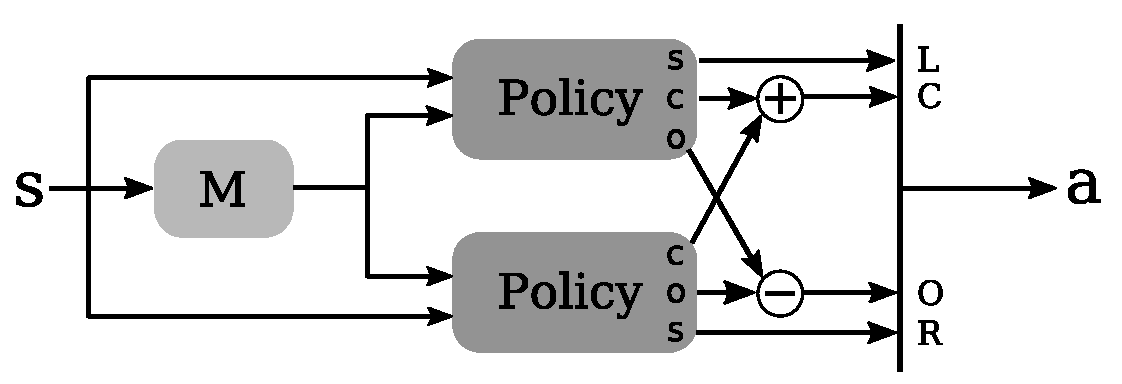
\includegraphics[width=0.9\columnwidth]{symmetry_figures/net_architecture_2.pdf}
  \caption{A universal method for converting any neural network into a symmetric network policy.}{$\mathcal{M}$ block is an environment-dependent state mirroring function. The two policy blocks are the same neural network module, with the output terminals re-order for illustration clarity.  The \textit{s, c, o} terminals corresponds to \textit{side}, \textit{common}, and \textit{opposite} joints as described in \Cref{sec:mirroring-functions}.}
  \label{fig:net-architecture}
\end{figure}

Another approach towards enforcing symmetry is to impose symmetry at the network architecture level. 
The goal here is to choose a network architecture such that \Cref{eq:symmetric-policy} 
holds for all states~$s$ and all network parameters~$\theta$.
There are multiple ways to go about designing such an architecture.
However, they may require some knowledge about how the actions and/or states 
in which case having access to the mirroring functions $M_s$ and $M_a$ is strictly-speaking not enough.

A general case description of this method would be lengthy, and thus we focus only on the key aspects here. 
The simplest case occurs when we can assume that the action vector is simply divided 
into two, one corresponding to each side of the body, 
and that the actions of one side can readily be applied to the other side through a simple swapping operation.
This ignores the common parts such as the torso and the head for the time being.
More concretely, consider:
\begin{align*}
    a &= \begin{bmatrix}a_l\\a_r\end{bmatrix} \\
    M_a(a) &= \begin{bmatrix}a_r\\a_l\end{bmatrix}
\end{align*}
where $a_l$ and $a_r$ are vectors of equal size.
In this case, we can define a symmetric policy composed of an inner network $f$ as follows:
\begin{align*}
    \pi_{side}(s) = \begin{bmatrix}
    f(s,M_s(s))\\
    f(M_s(s),s)\\
    \end{bmatrix}
\end{align*}
It is easy to show in this case that \Cref{eq:symmetric-policy} holds:
\begin{align*}
    \pi_{side}(M_s(s)) &= \begin{bmatrix}
    f(M_s(s),M_s(M_s(s)))\\
    f(M_s(M_s(s)),M_s(s))\\
    \end{bmatrix}\\
    &= \begin{bmatrix}
    f(M_s(s),s)\\
    f(s,M_s(s))\\
    \end{bmatrix}\\
    &= M_a\left( \begin{bmatrix}
    f(s,M_s(s))\\
    f(M_s(s),s)\\
    \end{bmatrix} \right)\\
    &= M_a\left(\pi_{side}(s)\right)
\end{align*}

When the action space also includes actions for common parts,
i.e., those such as the torso and head that have no symmetric counterparts,
it is easy to define $\pi_{com}(s) = h(s) + h(M_s(s))$ 
which is then invariant to left/right mirroring. 
Finally, the policy is then a combination of the common actions and side actions:
\begin{align*}
    \pi_\theta(s) = \begin{bmatrix}
        \pi_{com}(s)\\
        \pi_{side}(s)\\
    \end{bmatrix}
\end{align*}
Please refer to \Cref{fig:net-architecture} for an illustration of the NET method.

A drawback of this method is that it requires knowledge about the state and action symmetry structures to redefine the network. 
Also, this method is highly sensitive to state and action normalization.
The problem is that an ordinary normalization based on past experiences may break the symmetry.
Though the other methods introduced here can also suffer from the same problem, this method is much more sensitive to the issue.

\subsection{Practical Considerations}

There are some practical considerations to take into account when working with 
each of the methods introduced in the previous section.
In terms of implementation, the DUP and PHASE methods are the easiest to 
implement as they required little to no change to the learning pipeline.  
Architecture-based mirroring (NET)
requires the most modification to both the learning pipeline and the environments.
The LOSS method is the only approach here that allows us to balance the desire for symmetry 
with the original learning objective, albeit at the cost of an extra hyper-parameter.  
The NET method produces a truly symmetric policy, which is not possible with the other methods.
The PHASE method is the approach best suited for coping with neutral states, 
which represent symmetric states where it may become problematic to break symmetry.
We revisit this point later.
PHASE is also restrictive in that it enforces a predefined walk cycle timing.

%% normalization 

One more consideration relates to the application of normalization to network inputs, which is commonly done by 
using statistics gathered from the data itself.  
However, this can break some of the mirroring assumptions.  
The problem is most severe when using a symmetric network architecture, although other methods are
also impacted.
Fortunately, developing a normalization scheme that works correctly is relatively straightforward. 
A simple approach is to duplicate the states (or actions) as in \Cref{subsec:dup_epx} 
and to compute the statistics based on the aggregated set of states (or actions) and 
their mirrored states (or actions).



\section{Gait Symmetry Metrics}
\label{sec:metrics}

All of the methods discussed only provide indirect paths, via the learned policies, 
for achieving symmetry for the actual motions. 
Therefore it is important to evaluate how well these methods do at achieving their final goal. 
\citeauthor{Yu-SIGGRAPH-2018}\cite{Yu-SIGGRAPH-2018} uses an established metric in the biomechanics literature 
known as the Robinson Symmetry Index (SI):
\begin{align}
    SI = \frac{2|X_R - X_L|}{X_L + X_R}\cdot 100,
\end{align}
where $X_R$ is a scalar features of interest, such as the duration of the stance phase 
for the right leg, and $X_L$ is its counterpart for the left leg. 
Previous work using the LOSS method~\cite{Yu-SIGGRAPH-2018} chooses to use the average actuation 
magnitude as the parameter of interest which leads to $X_R = \sum_{t=1}^T \norm{\boldsymbol{\tau}_{t,R}}_2$ where $\boldsymbol{\tau}_{t,R}$ is the vector of applied torques at time $t$ for the right leg. 
We will refer to this as the \textit{actuation symmetry index (ASI)}.
In practice, we found that the ASI can be misleading in some circumstances, 
e.g., a high torque applied to the right hip can be conflated with a high torque applied to the left knee, 
which is not desirable. ASI also loses information about signs of the applied torques.

The \textit{phase-portrait} is another tool that can be used to qualitatively investigate 
the symmetry or asymmetry of a gait, as seen in \cite{symmetry_phase_portrait}. 
The phase-portrait is a scatter plot drawn over a period of time, usually over a single gait cycle.
The $x$ and $y$-axes of the 2D plot correspond to the position and velocity, respectively, of a joint of interest, 
such as the hip flexion, 
For an asymmetric gait, the phase portraits of the two sides will not fully overlap.
To numerically quantify the similarity between two phase-portraits, we propose to use a~\textit{phase-portrait index} (PPI).  
One problem to address is that the left and right limbs usually have a phase offset even for a symmetric motion.
This is not a problem when inspecting the phase-portraits visually, but the problem needs to be addressed to compute a 
meaningful metric.
We solve this by finding the best phase offset between the left and the right side through an exhaustive search. 
We also normalize each axis so that $x,y\in[-1,1]$ to address the potential discrepancy between magnitudes of different gaits.
The final PPI is defined according to:
\begin{align}
    PPI = \frac{1}{C} \min_s \sum_{t=0}^{C-1} \norm{q_t^R - q_{t+s}^L}_1 + \norm{\dot{q}_t^R - \dot{q}_{t+s}^L}_1,
\end{align}
where $C$ is the length of a gait cycle, $q_t^R$ and $\dot{q}_t^R$ are the normalized right joint 
position and velocity at time $t$. Similarly, $q_{t+s}^L$ is the normalized left joint position 
at time $t+s$ modulo $C$, as the elements that are shifted beyond the last position are reintroduced at the beginning.

\section{Environments}
\label{sec:environments}
\begin{figure}%
  \centering
  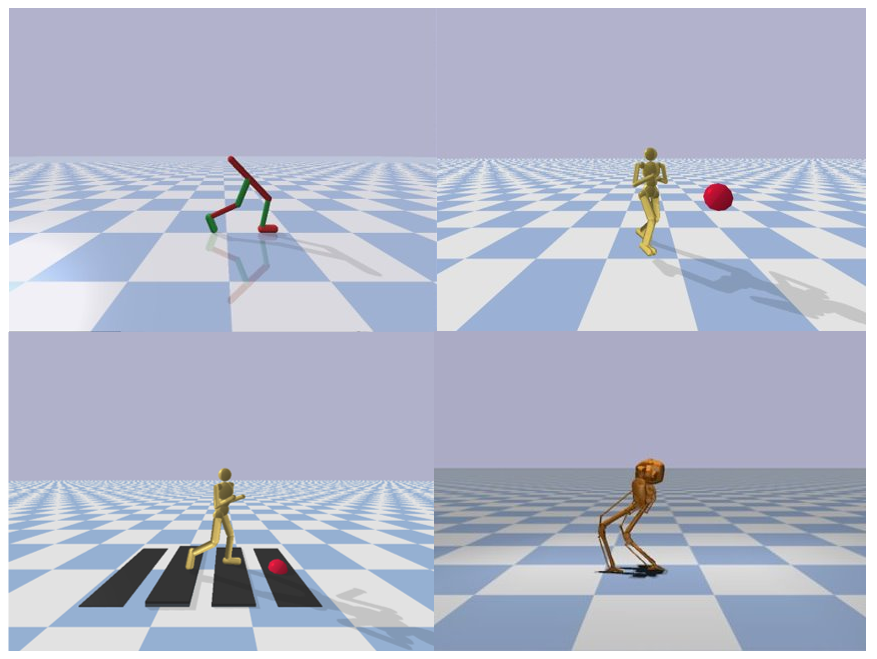
\includegraphics[width=0.9\columnwidth]{symmetry_figures/task_overview_2.png}
  \caption{Environments.}{Top-left: {\it Walker2D}. Top-right: {\it Walker3D}. Bottom-left: {\it Stepper}. Bottom-right: {\it Cassie}.}
  \label{fig:task-overview}
\end{figure}

We evaluate the effectiveness of the enforcement methods described in \Cref{sec:methods} 
on four different locomotion tasks, i.e., RL ``environments''.  
The environments were chosen to represent a fairly diverse range of locomotion tasks.  
They are described in detail below.  
For each environment, we run each method 5 times and plot the mean results.

\bfpara{Walker2D} The implementation of {\it Walker2D} environment is taken directly from PyBullet \citep{ref:Pybullet} 
without further modification. This character is almost identical to the one used in \Cref{sec:params_torque}. The purpose of this environment is to evaluate each symmetry method on 
a well-established existing reinforcement learning environment.  
The task is for the character to walk as far as possible in the forward direction in the allotted time.  
An action is a 6D vector corresponding to a normalized torque at each of the hip, knee, and ankle on both left and right legs.  
The observation space is~22D and consists of root information (root z-coordinate, x and y heading vector, root velocity, 
roll, and pitch), joint angles, joint angular velocities, and binary foot contact information.

\bfpara{Walker3D}  This represents a 3D character simulated in PyBullet, with targets randomly placed, at a distance,
in the half-plane in front of the character.  
The task requires character to navigate towards the target and then stop at the target.  
A new target will be chosen, in the forward half-plane of the current character orientation, 
once the target is reached and one second has passed.  
The 3D character has 21-DoF corresponding to abdomen (x3), hip (x3), knee, ankle, shoulder (x3), and elbow.  
The observation space is 52D, and is analogous to that provided for {\it Walker2D},
with an additional 2D vector representing the target location in the character root frame.

\bfpara{Stepper}  {\it Stepper} uses the same model as \textit{Walker3D}, and 
requires it to navigate terrain consisting of a sequence of stepping blocks.  
The blocks are randomly generated by sampling from the following distributions:
spacing $d \sim \mathcal{U}(0.65, 0.85)$ meters and height variation of the next step $h \sim \mathcal{U}(\text{-}25, 25)^{\circ}$.  
The character receives information for two upcoming blocks as an $(x,y,z)$ offset in character root space.  
The stepping block information advances when either foot contacts the immediate next block, 
which effectively forces the character to step precisely on each step.  
The precise foot placement requirement, as well as variable terrain height, makes this environment 
more challenging than \textit{Walker3D}.

\bfpara{Cassie}  The task requires a bipedal robot Cassie to walk forward at a desired speed 
while mimicking a reference motion.  Since the reference motion is time-indexed, the character receives a phase variable as input.  
The phase variable varies according to $\phi \in [0,1)$ in the gait cycle.  
In addition to phase, the character receives other inputs including the height, the orientation expressed as a unit quaternion,
pelvis velocities, angular velocities, and acceleration, joint angles and angular velocities.  
In total, the Cassie robot has a 10D action space and 47D observation space.  
Another important distinction between {\it Cassie} and the other tasks is that it is implemented in 
MuJoCo~\citep{ref:Mujoco}, while other environments use the Pybullet~\citep{ref:Pybullet} physics engine. 
This simulated model has also been validated to be close to the 
physical Cassie robot~\cite{cassie-sim-to-real}.


\section{Results}

We compare the four methods, together with an asymmetric baseline, across four different 
locomotion tasks of varying difficulties\footnote{The source code is available at \url{https://github.com/UBCMOCCA/SymmetricRL}.}.

\subsection{Summary}

We begin with a high-level summary of our findings.  All symmetry enforcement methods improve motion quality over the baseline, but they cannot be reliably ranked across different environments.  In general, DUP is the least effective in enforcing symmetry, while LOSS is the most consistent.  For imitation-guided tasks, where the reward is related to imitating a time-indexed reference motion, such as for \textit{Cassie} and \textit{DeepMimic}, the PHASE method appears to be superior.  

Regarding learning speed, the symmetry enforcement methods have no consistent and predictable impact, positive or negative.  While this contradicts our initial expectation, it does not provide the full picture.  In particular, even though BASE achieves relatively high rewards in \textit{Stepper}, it was unable to make forward progress in any of the five runs.  In summary, we suggest symmetry methods be used for producing higher quality symmetric motions, i.e., closer to what we might expect from human and animal movement, but not necessarily for faster learning.  We further expand the comparison of the different methods in two sections below.

\subsection{Effect on Learning Speed}

One of our initial hypotheses was that the learning speed can be improved by enforcing symmetry.  
Symmetry can be considered as domain knowledge that may otherwise be difficult to learn, 
especially considering its abstract nature.  
However, our experiments indicated that enforcing symmetry, in general, has no consistent impact on the learning speed.
As shown in \Cref{fig:learning-curves}, BASE performs well in \textit{Walker2D} and \textit{Walker3D}.  
In particular, although BASE was not initially the fastest in \textit{Walker3D}, 
it ultimately achieves a higher return than all mirroring methods.  
On the other hand, BASE fails to learn the \textit{Stepper} task in all five runs;
it often pauses near the beginning without taking a single step.  
This is consistent with findings by \citeauthor{Yu-SIGGRAPH-2018}, 
who also find that symmetry enforcement can be crucial when learning more difficult tasks.

For the \textit{Cassie} environment, the benefit of enforcing symmetry is evident 
because the reward explicitly encourages the character to imitate a symmetric reference motion.  
We hypothesize that for such a case, symmetry suitably constrains the search space 
for the symmetric task. However, if symmetry is not rewarded, explicitly or implicitly, 
then its effects may not be reflected in the learning curve.  Finally, between the symmetry methods, 
there is no clear winner in terms of learning speed.

\begin{figure*}[tbh]
  \centering
  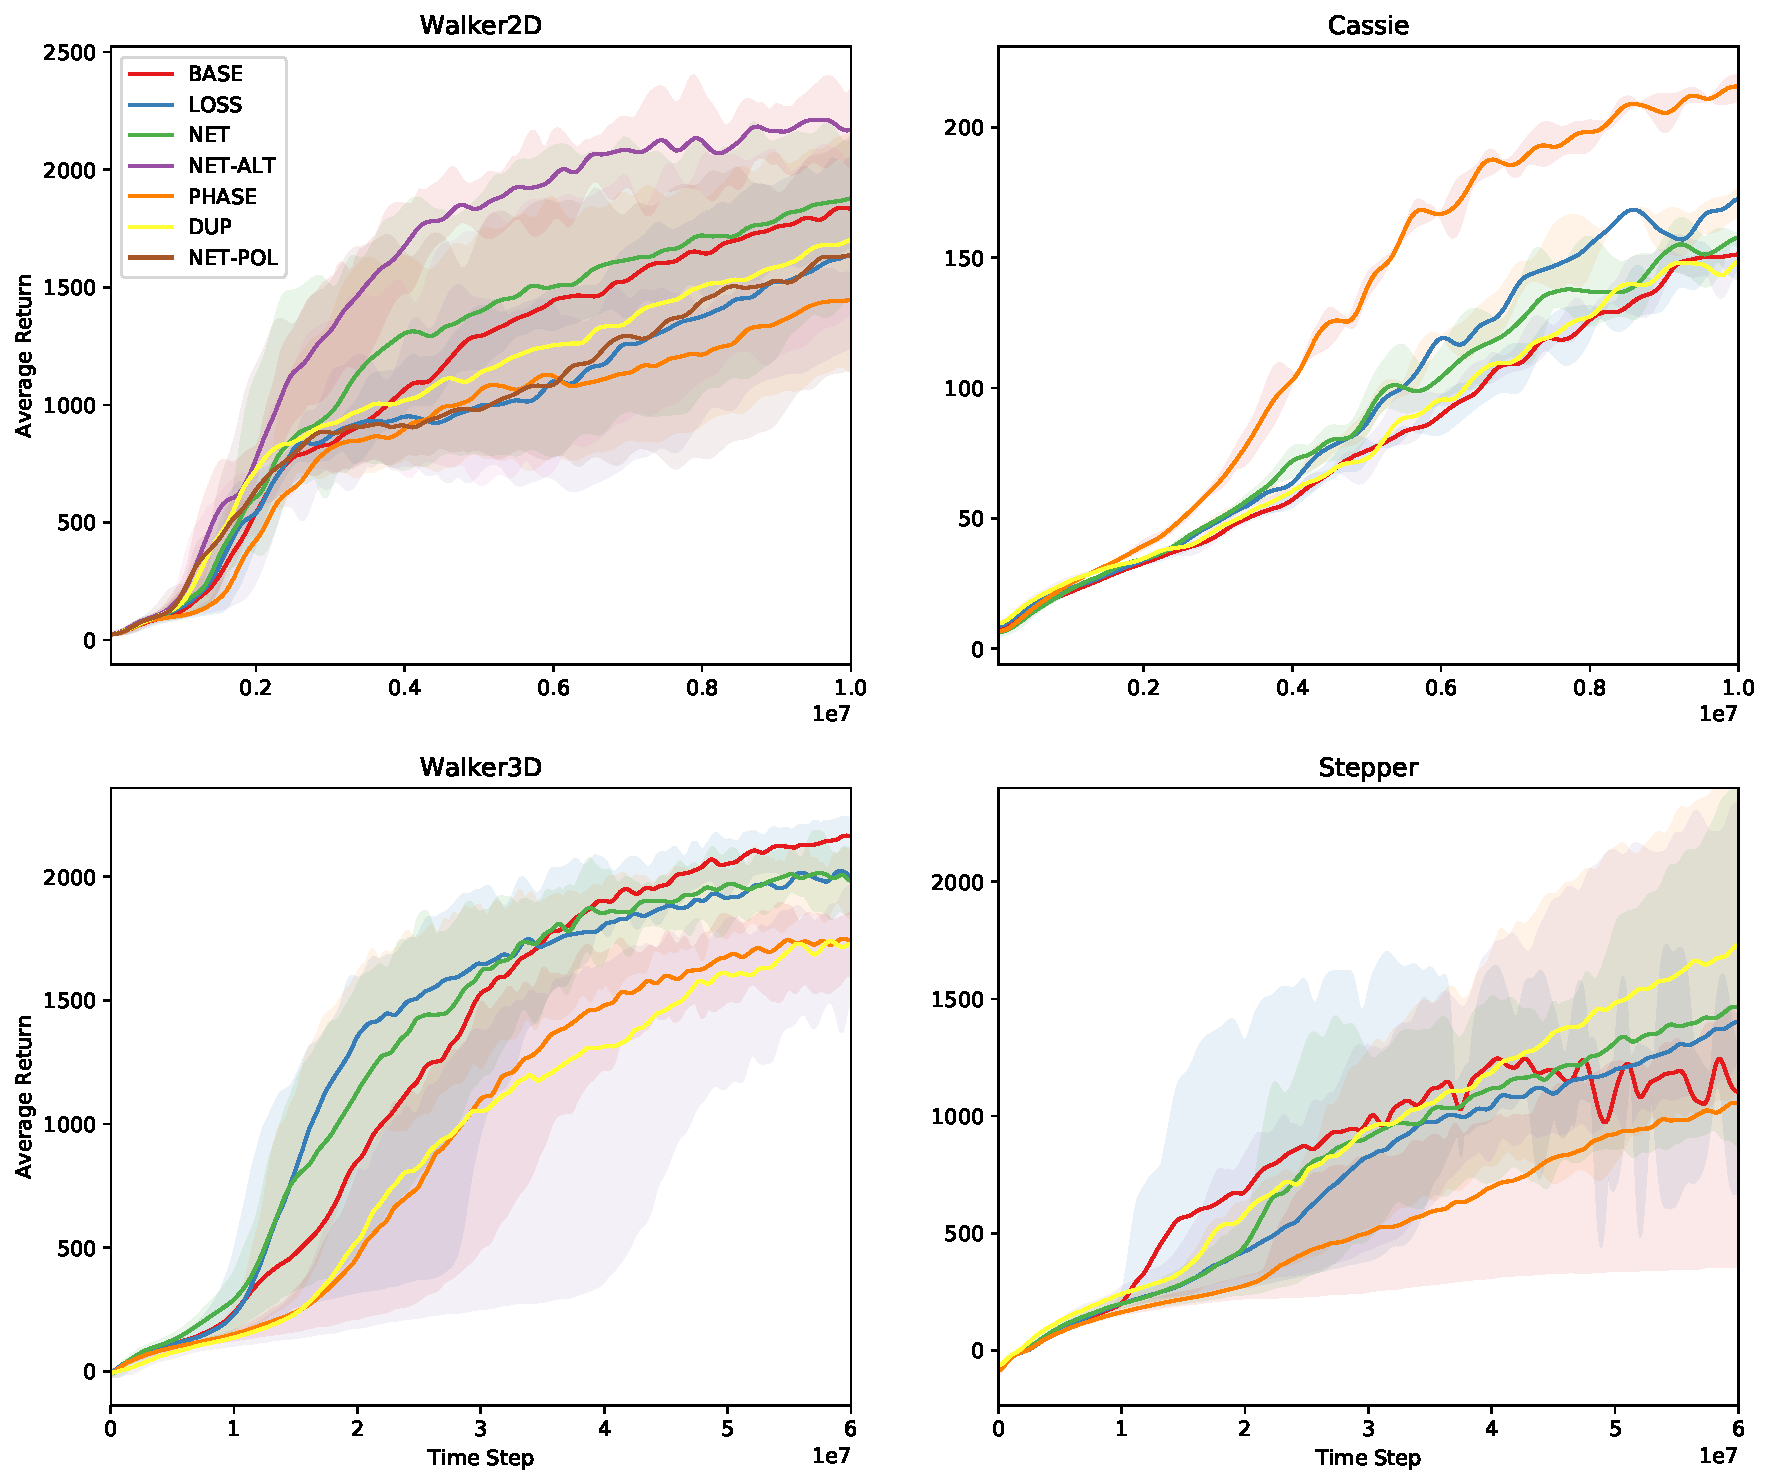
\includegraphics[width=\columnwidth]{symmetry_figures/LearningCurves.pdf}
      \caption{Learning curves for different symmetry methods in each of the four locomotion environments (\Cref{sec:environments}).}{The \textit{Walker2D} plot contains two additional experiments aside from the baseline and four symmetry methods.  \textit{NET-ALT} uses an alternate formulation of symmetric network architecture described in \Cref{sec:alternate-network}.  \textit{NET-POL} is an ablation study on \textit{NET} with symmetry enforcement only on the policy network and not on the value network.}
  \label{fig:learning-curves}
\end{figure*}

\begin{figure*}[tbh]
  \centering
  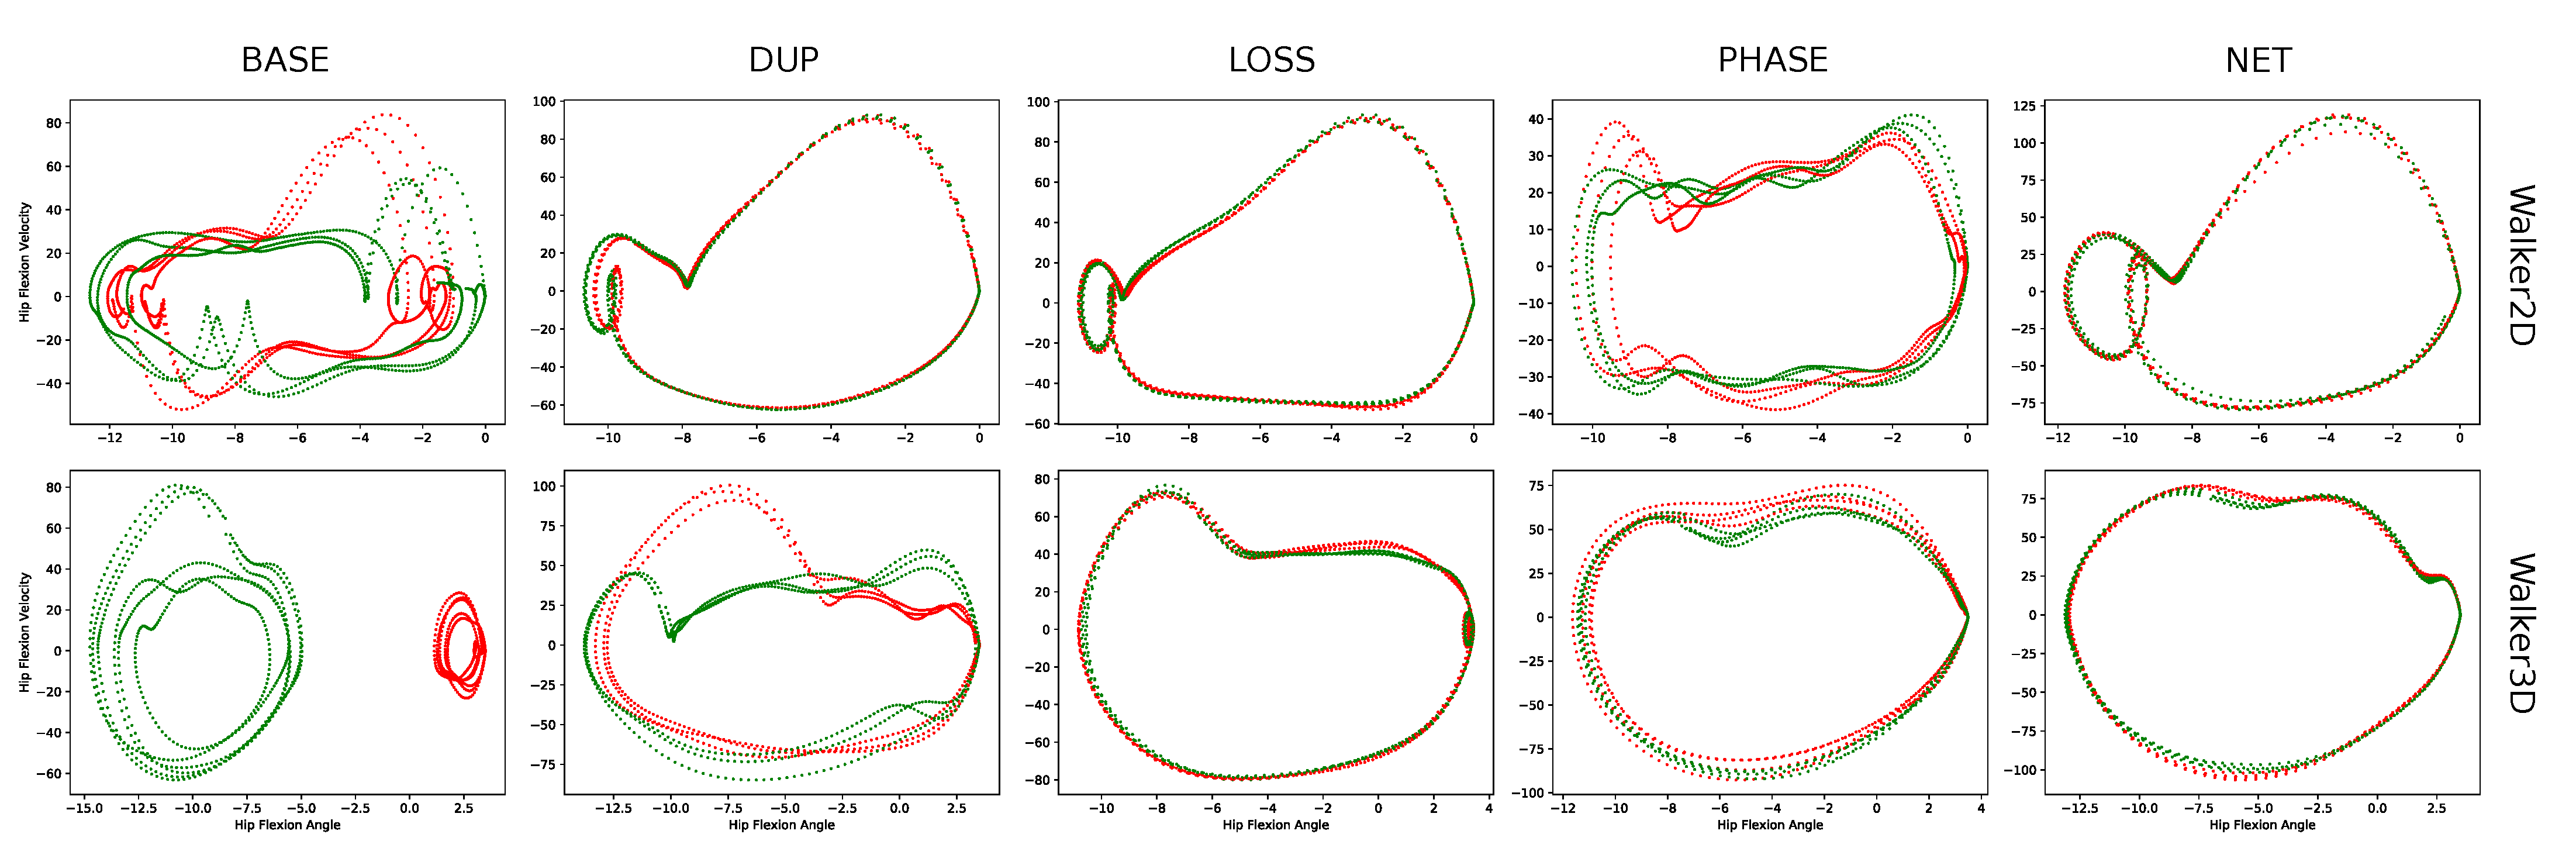
\includegraphics[width=\columnwidth]{symmetry_figures/phase_plots_smaller.pdf}
  \caption{Phase-portrait for \textit{Walker2D} and \textit{Walker3D}.  The green curve is for the left hip flexion and red for the right side.  The more symmetric the motion, the more aligned are the curves.}
  \label{fig:phase-portraits}
\end{figure*}


\bfpara{PHASE and Imitation-Guided Learning}  In phase-based symmetry experiments, 
we define a phase variable in correspondence to the gait cycle.  
For the \textit{Cassie} environment, we use a period of 0.8~s, 
which is determined based on the reference motion.  
For all other environments, we assign a period based on a working solution.

We find phase-based symmetry enforcement to be effective for imitation-guided learning, 
as it outperforms other methods by a significant margin for \textit{Cassie}.  
When comparing \textit{Cassie} with \textit{DeepMimic}~\cite{2018-TOG-deepMimic}, 
which also uses an imitation objective, we find the results to be consistent.  
The learning curves for our \textit{DeepMimic} symmetry experiment are presented in \Cref{sec:deepmimic-results}.  
We hypothesize that phase-based symmetry is effective for imitation-guided tasks when
the motion clips used for training containing suitably-periodic and symmetric motions.  
On the other hand, PHASE constrains the period of the gait cycle, 
which can be harmful for non-imitation tasks. 
PHASE performs poorly in terms of learning speed 
when used without a reference motion, i.e., 
for \textit{Walker2D}, \textit{Walker3D}, and \textit{Stepper}, although
it can do well in terms of quality, e.g., for \textit{Walker3D}.

\bfpara{Alternate Symmetric Network}  The NET method presented in \Cref{fig:net-architecture} is 
an intuitive way of converting any neural network into a symmetric policy.  
However, it is perhaps not the immediate solution that one would come up with when tasked to design a symmetric neural network.  
We include one of our earlier constructions of symmetric policy in \Cref{sec:alternate-network}, 
which we refer to as NET-ALT.  A major difference between NET and NET-ALT is that the latter uses 
shared weights at the layer level to explicitly enforce the symmetry constraint in \Cref{eq:symmetric-policy}.  
Despite this, the two architecture-based mirroring methods should, in theory, have similar performance.  
As can be seen in \Cref{fig:learning-curves}, NET-ALT significantly outperforms NET in the \textit{Walker2D} environment, 
along with the baseline and all other mirroring methods.  
We believe that the structure of the symmetric layer matrix in \Cref{sec:alternate-network} 
may be the key to resolve this gap, which remains to be verified.

\bfpara{Policy Network Ablation Study}  As an ablation study, we removed the symmetry constraint 
for the value network in the NET method.  Since our goal is to produce a symmetric policy, 
and the value network is discarded after training, we want to see how enforcing symmetry in the value network 
during training affects the learning speed.  In \Cref{fig:learning-curves}, the two curves of interest are 
NET and NET-POL, where the latter has the symmetry constraint removed for the value network.  
Our experiment shows that it is beneficial to enforce the symmetry constraint for the value network during training
since the difference between the curves is not insignificant.  

\subsection{Symmetry Enforcement Effectiveness}

Although learning speed is a major point of interest from the ML perspective, 
our work is nevertheless motivated by the aesthetics of symmetric gaits that are needed for applications in animation.  
We measure the effectiveness of each symmetry enforcement methods on the metrics we defined in \Cref{sec:metrics}.  
In most cases, we find that symmetric gaits are better achieved when any of the enforcement methods are applied, 
as compared to the baseline.  The motions produced by the symmetry methods are also more 
natural-looking, subjectively speaking, than without mirroring.

\Cref{fig:phase-portraits} shows the phase-portraits for \textit{Walker2D} and \textit{Walker3D}.  The symmetry metrics for all environments are summarized in \Cref{tab:actuation_si} and \Cref{tab:pp_msi}.
To perform consistent measurement for the metrics, we omit the first two strides to limit the influence of the transition period from standing to locomotion.  
The reported metrics are calculated from the median of the ten subsequent strides after the initial two.  
For the \textit{Stepper} tasks, we use the median from five strides to accommodate for the increased difficulty.  
Also, note the \textit{Stepper} results are missing for BASE because it was unable to produce 
consistent gait cycles that can be measured.  In most cases, the policy either learns to pause 
at the starting location or falls after taking one or two steps.

As in learning speed, there is not a single best mirroring method across all environments.  
However, from the overall picture, we found that LOSS and PHASE to be the most consistent among all methods.  
In general ASI and PPI do not agree on a single best method except for the \textit{Cassie} task where PHASE is the best.


\begin{table}[tbh]
    \centering
    \begin{tabular}{l|c|c|c|c}
    & Walker2D & Walker3D & Stepper & Cassie  \\
    \hline
    BASE & \textit{3.97} & 6.36 & \xmark & 9.27   \\
    DUP & 3.77 & 7.57 & 7.54 & 6.58   \\
    LOSS & 2.56 & 4.48 & 6.36 & \textit{15.72}   \\
    PHASE & 3.77 & \textbf{2.55} & \textbf{3.99} & \textbf{4.49}   \\
    NET & 2.00 & \textit{10.64} & \textit{28.97} & 5.15   \\
    NET-ALT & \textbf{1.04} & -- & -- & --   \\
    NET-POL & 1.71 & -- & -- & --   \\
    \end{tabular}
    \caption{Actuation SI. Lower numbers are better.}
    \label{tab:actuation_si}
\end{table}


\begin{table}[tbh]
    \centering
    \begin{tabular}{l|c|c|c|c}
    & Walker2D & Walker3D & Stepper & Cassie  \\
    \hline
    BASE & \textit{1.06} & \textit{2.16} & \xmark & \textit{0.49}   \\
    DUP & 0.39 & 1.61 & 0.57 & 0.41   \\
    LOSS & 0.33 & \textbf{0.19} & \textbf{0.46} & 0.31   \\
    PHASE & 0.57 & 0.30 & 0.49 & \textbf{0.17}   \\
    NET & \textbf{0.16} & 0.58 & \textit{0.65} & 0.23   \\
    NET-ALT & \textbf{0.16} & -- & -- & --   \\
    NET-POL & 0.28 & -- & -- & --   \\
    \end{tabular}
    \caption{Phase-portrait index. Lower numbers are better.}
    \label{tab:pp_msi}
\end{table}



\section{Discussion}

Symmetry can sometimes be harmful, especially when the character begins from or otherwise arrives at a neutral pose,
i.e., a symmetric pose where $s = M_s(s)$.  The problem is that a symmetric policy is incapable of escaping 
from a neutral pose since the action that it takes would also be symmetric.  
When a symmetric action is applied in a symmetric state, the next state is necessarily also symmetric.  
For instance, a character that starts from the T-pose will likely perform some kind of hopping gait, 
since the feasible locomotion possibilities which perpetuate symmetric states and actions are limited.  
To make matters worse, states near the neutral states can also become problematic.

The breaking symmetry problem is most severe when enforcing symmetry through network architecture, as this method is guaranteed to produce true symmetric policies.  While DUP and LOSS methods can suffer from the same issue, they can implement workarounds at an additional cost.  This issue, however, does not affect PHASE.
A simple workaround to this problem is to always start the character from a non-neutral position.  This can be easily achieved by adding some random noise to each joint of the initial pose at the start of the task.  In practice, we did notice that
on occasion the character would converge on a hopping gait. However, the simple workaround works well 
for the majority of cases in our experiments.

% \subsection{Is Perfect Symmetry Always Desirable?}

Our work is motivated by the premise that healthy human gaits are usually symmetric.  
However, this remains a controversial issue in the biomedical literature~\cite{riskowski, SADEGHI200034}.  
The strongest argument for asymmetry in human motor control is the general belief that humans have a dominant side that is often the preferred choice for manipulating objects.  This is also tied with the need for a leading foot to start a walk or run cycle in the neutral state problem.  One should, therefore, be aware of the implications when enforcing perfect symmetry.
Quadrupedal locomotion, which has six commonly observed gaits as opposed to the three gaits of bipeds \cite{locomotion_mcmahon}, is also interesting to examine.  Of these six, half are fairly symmetric including walk, trot, and rack. However, the remaining three, also known as the in-phase gaits which are used at high speeds, are often asymmetric. Since the symmetry of gait and policy are not the same, it would be interesting to see whether it is possible to nevertheless 
achieve these non-symmetric quadrupedal gaits with a symmetric policy.

\section{Conclusions}

In this chapter, we explore the use of symmetry constraints for DRL-based learning of locomotion skills.
We compared four different enforcement methods, in addition to a symmetry-free baseline, 
across four different locomotion tasks of varying difficulty.  
We find that enforcing symmetry constraints can sometimes be harmful to learning efficiency,
but that in general, it produces higher quality motions. When comparing the symmetry methods, we find that the results, both in terms of learning speed and motion symmetry, 
to be environment-dependent.  A notable exception is that the phase-based mirroring method generally 
performs better than the baseline for imitation-guided reward settings such as for \textit{Cassie} and \textit{DeepMimic}.

The difference between the enforcement methods is more pronounced from the implementation standpoint.  
LOSS and PHASE methods have the burden of an additional hyperparameter to tune. 
However, the additional parameter can also be viewed as an advantage in terms of flexibility.  
In LOSS, the hyperparameter can be used to adjust the strength of symmetry constraint.  
For PHASE, the phase variable allows us to define a desired locomotion period. 
Given the similarities across all methods, it is perhaps justifiable to choose one based on the implementation overhead.  
DUP is the easiest to implement and evaluate since it requires minimal change to the
existing RL pipeline and has no hyperparameter to tune.  
Finally, if the application requires absolute symmetry, then the NET method is guaranteed to produce a symmetric policy.

The application of symmetric policies is not limited to locomotion.  
Many classical control tasks may benefit significantly from leveraging symmetry, 
including acrobat, cart-pole, and pendulum \citep{ref:OpenAI-Gym}.  
Furthermore, the notion of symmetry extends beyond left-right symmetry and even character motion.  
The Sudoku game is an example task that exhibits multiple types of symmetry properties. 
Whether a learning method can take full advantage of all the symmetries remains an open question.
However, this paper lays a foundation for enabling future studies on inductive biases
based on symmetry.
%\chapter{RL in the Real World: Cassie}
\label{ch:cassie}
...
\chapter{Conclusions}
\label{ch:conclusions}

Reinforcement learning provides a promising new path for motion generation, one that can be generalized to new terrains and character morphologies effortlessly. However the current methods are computationally inefficient and unless motion captured data is used the motion quality is commonly unsatisfactory for applications in computer graphics.

This work tries to tackle these two problems by investigating two of the usual suspects, the excessively large torque limits and gait asymmetry. We show that more realistic torque limits, though resulting in more natural motions, can hinder the training in the beginning. We propose to use a simple curriculum learning technique that starts with higher torque limits to speed up the training but gradually decreases the limits to arrive at more natural final motions. This way we get the best of both worlds.

Next, we looked at ways of incorporating gait symmetry into the training process. Symmetric motions are generally perceived to be more attractive in humans and asymmetric patterns are commonly associated with disability or injury. We have compared four methods of enforcing symmetry on various environments as well as discussing their advantages and drawbacks in different scenarios.
%\chapter{Related Work}
\label{ch:relatedwork}


\section{Motion Symmetry}
Motion symmetry has been a topic of interest for many years in the study of human motion and movement biomechanics. 
Symmetric motions are perceived to be more attractive, e.g., for dance~\cite{danceSymmetry},
and gait symmetry is seen an as a desirable outcome for physiological manipulation~\cite{robinson1987use}.
While symmetry is a common assumption in the study of gait and posture, 
individual gaits often do exhibit asymmetries due to various possible functional causes~\cite{seelet}.
We refer the reader to a past review article~\cite{SADEGHI200034} for insights
into the degree of symmetry of lower limbs movement during able-bodied gait
and the potential influence of limb dominance on the motion symmetry of the lower extremities.
and human gaits~\cite{riskowski}.
It is also not obvious how to best quantify 
the asymmetry of human gaits, and thus specific symmetry metrics have been
proposed~\cite{symmetry_measures,symmetry_phase_portrait}.

The robust control of physics-based character locomotion has been a long-standing challenge
for character animation. We refer the reader to a survey paper for a detailed history~\cite{STAR2012}.  
An early and enduring approach to controller design has been to structure control policies around finite state
machines (FSMs) and feedback rules that use a simplified abstract model or feedback law.  These general
ideas have been applied to human athletics and running~\cite{Hodgins95} and a rich variety of walking
styles~\cite{Yin07,Coros10,LeeYS10}. Many controllers developed for physics-based animation
further use optimization methods to improve controllers developed around an FSM-structure, or use an FSM to 
define phase-dependent objectives for an inverse dynamics optimization to be solved at each time step.
Policy search methods, e.g., stochastic local search or CMA~\cite{Hansen06}, can be used to optimize the 
parameters of the given control structures to achieve a richer variety of motions, e.g.,~\cite{Yin07,Coros11}, and
efficient muscle-driven locomotion~\cite{Wang09}.  
Many of the FSM controllers use hard-coded symmetries, which assign the roles of stance-leg or swing-leg
to the left and right legs, as a function of the FSM state.
It is common in kinematic-based approaches to locomotion, e.g.,~\cite{bruderlin,HoldenPFNN}, 
to also mirror all the available motion data
in order to double the effective size of the data set, and to reflect the often-symmetric nature of human locomotion.
Lastly, trajectory optimization-based methods also commonly assume motion symmetry when convenient, e.g.,~\cite{majkowska2007flipping}.

More recently, locomotion synthesis has attracted significant
attention from the reinforcement learning (RL) community, where the OpenAI Gym tasks have 
become a popular RL benchmark~\cite{ref:OpenAI-Gym}. In this context, symmetry constraints are commonly 
not imposed, and the resulting motions often have noticable asymmetries. 
Further work extends these efforts in a variety of ways, including the traversing challenging terrains~\cite{ref:deepmindParkour}.
More realistic and dynamic motions can be achieved with the help of 
motion-capture clips~\cite{2017-TOG-deepLoco,2018-TOG-deepMimic} and these use
what we refer to as the PHASE symmetry method with the goal of more efficient learning, although with
no robust documented experiments to verify the efficiency gains.
The efficient learning of controllers capable of producing high-quality motion for realistic-strength characters remains
a challenging problem in the absence of motion capture data. Recent work makes
progress on this problem using RL with a combination of energy optimization, learning curriculum, and 
an auxiliary motion symmetry loss~\cite{Yu-SIGGRAPH-2018}, which we shall refer to as the LOSS method.

A recent result investigates how DRL problems can become prone to learning plateaus because
of winner-take-all solution modes~\cite{ray_interf}. These can easily arise in DRL because the distribution of data
for policy learning is directly influenced by the policy itself. Thus in the case of multiple diverging 
decision paths, one of the modes will quickly dominate. The choice of whether to encourage symmetry,
and how to do so, may create an optimization landscape that exhibits similar properties.

%\include{model}
%\include{impl}
%\include{discussion}
%\chapter{Conclusions}
\label{ch:conclusions}

Reinforcement learning provides a promising new path for motion generation, one that can be generalized to new terrains and character morphologies effortlessly. However the current methods are computationally inefficient and unless motion captured data is used the motion quality is commonly unsatisfactory for applications in computer graphics.

This work tries to tackle these two problems by investigating two of the usual suspects, the excessively large torque limits and gait asymmetry. We show that more realistic torque limits, though resulting in more natural motions, can hinder the training in the beginning. We propose to use a simple curriculum learning technique that starts with higher torque limits to speed up the training but gradually decreases the limits to arrive at more natural final motions. This way we get the best of both worlds.

Next, we looked at ways of incorporating gait symmetry into the training process. Symmetric motions are generally perceived to be more attractive in humans and asymmetric patterns are commonly associated with disability or injury. We have compared four methods of enforcing symmetry on various environments as well as discussing their advantages and drawbacks in different scenarios.

%    3. Notes
%    4. Footnotes

%    5. Bibliography
\begin{singlespace}
\raggedright
\bibliographystyle{abbrvnat}
\bibliography{biblio}
\end{singlespace}

\appendix
%    6. Appendices (including copies of all required UBC Research
%       Ethics Board's Certificates of Approval)
%\include{reb-coa}	% pdfpages is useful here
\setcounter{chapter}{-1}
\chapter{Supporting Materials}
\renewcommand{\thechapter}{A}

% This would be any supporting material not central to the dissertation.
% For example:
% \begin{itemize}
% \item additional details of methodology and/or data;
% \item diagrams of specialized equipment developed.;
% \item copies of questionnaires and survey instruments.
% \end{itemize}

% \section{Symmetric Locomotion}


% \section{\Cref{ch:envparams} Hyper-parameters}
\section{Chapter 4 Hyper-parameters}
\label{sec:envparam_hyperparams}

The following contains the hyper-parameters used for all of the experiments in \Cref{ch:envparams}. The code is also available under \url{https://github.com/farzadab/walking-benchmark/}.
\begin{table}[h]
    \centering
    \begin{tabular}{lc}
        \toprule
        Name & Description \\
        \midrule
        Policy LR & $3e^{-3}$\\
        Value Network LR & $5e^{-3}$\\
        Total Environment Steps & $6$ Million\\
        Clipping Parameter ($\epsilon$) & $0.2$\\
        Decay ($\gamma$) & $0.99$\\
        GAE $\lambda$ & $0.95$ \\
        Policy type & Fixed Diagonal Gaussian\\
        Policy stdev & $\exp(-1)$\\
        Network Size & 3 Layers of 256 nodes \\
        Network Activations & ReLU \\
        Max Grad Norm & 1\\
        Optimization Batch Size & $128$ \\
        PPO Optimization Steps & $10$ \\
        \bottomrule
    \end{tabular}
    \caption{Hyper-parameters used in \Cref{ch:envparams}.}
    \label{tab:envparam_hyperparams}
\end{table}

\section{Mirroring Functions}
\label{sec:mirroring-functions}

The mirroring functions, $\mathcal{M}_s$ and $\mathcal{M}_a$ as described in \Cref{sec:methods} are properties of the environment.  Consequently, the environment is responsible for providing the necessary information for policies to perform the mirroring operation on state and action.  Although the mirroring functions can be arbitrarily complex, we found that all the environments in \Cref{sec:environments} share a similar construction.  Using \textit{Walker3D} as an example, the method for deriving mirror functions are described in detail below.

The \textit{Walker3D} character has a total of 21-DoF and each DoF is modelled as a one-dimensional hinge joint.  Furthermore, let the \textit{x}-axis be the forward direction and the \textit{z}-axis pointing up in the local coordinate frame of the character.  For mirroring purposes, the joints can be divided into three categories, common, opposite, and side.  The common categories contain joints that are unchanged by the mirroring function, such as $abdomen_y$.  In general, joints that rotate about the \textit{y}-axis should remain unchanged after mirroring.  The opposite categories contain joints that are mainly on the torso of the character and they need to be negated for mirroring.  In the case of \textit{Walker3D}, only $abdomen_x$ and $abdomen_z$ would fall under this category.  The side categories contain joints that are on the limbs.  Importantly, for each joint on one side, there must be a corresponding joint on the other side; for instance, the right knee corresponds to the left knee.  With the one-to-one mapping, $\mathcal{M}_a$ can simply interchange the applied torques for the respective joints on either side.  We found that it is more straightforward if the joint rotation axes are flipped, except for axes aligned on the  \textit{y}-axis, for the left and right limbs.  Otherwise, additional negation operations need to be applied after interchanging left and right actions. 

$\mathcal{M}_s$ follows a similar pattern as described above.  For state information that is derived from the character, such as joint angles and angular velocities, the mirrored counterpart would have negated and interchanged values.  Besides, the environment may provide additional information, such as character orientation, velocity, and target location in character root space, as in \textit{Walker3D}.  For vector-valued information, such as velocity and target location, the values along the $y$-axis should be negated; for orientations, values representing roll and yaw should be negated.


\section{Alternate Symmetric Network Architecture}
\label{sec:alternate-network}

In \Cref{fig:net-architecture}, we presented a universal method for embedding any neural network into a symmetric policy.  The NET method effectively uses the same policy module twice with flipped inputs for $s$ and $M(s)$.  While this construction is relatively simple to implement, alternative symmetric policy constructions do exist.  In this section, we describe the construction used for NET-ALT in \Cref{fig:learning-curves}.



Recall that a symmetric policy is one that satisfies \Cref{eq:symmetric-policy}, along with the fact that our mirror functions (\Cref{sec:mirroring-functions}) essentially perform negation and swapping operation on the state and action vectors.  Let us then consider the individual layers of a neural network as matrix operations, in particular, before the application of non-linear activation functions.  The full matrix form of the first layer for $s$ and $\mathcal{M}_s(s)$ can be written as,

\begin{center}
$\begin{bmatrix} W \\ X \\ Y \\ Z  \end{bmatrix} = (a_{ij})_{4\times4} \begin{bmatrix} C \\ O \\ R \\ L \end{bmatrix}$ and, $\begin{bmatrix} W \\ -X \\ Z \\ Y  \end{bmatrix} = (a_{ij})_{4\times4} \begin{bmatrix} C \\  -O \\  L \\ R \end{bmatrix}$.
\end{center}

$C$, $O$, $R$, $L$ represent the portions of the state vector corresponding to common, opposite, right, and left respectively.  The uppercase letters for $C$, $O$, $R$, $L$, $W$, $X$, $Y$, and $Z$ indicate that these are not necessarily scalars. For instance, for \textit{Walker3D}, $O$ contains both $abdomen_x$ and $abdomen_z$.  Similarly, the matrix, $(a_{ij})_{4\times4}$, is dimensionally consistent with the corresponding elements in the state vector.  For example, $a_{2j}$ is a two-column wide block that matches with the two elements in $O$ for \textit{Walker3D}.  In addition, notice the negated $O$ and $X$, as well as the interchanged $R$ and $L$ are the effect of the mirroring functions.  Overall, there are a total of 16 unknowns and 8 equations.  A symmetric layer can be obtained by solving this system of equations.  In particular, \textit{NetAlt} contains symmetric layers of the following form,

\begin{center}
$(a_{ij})_{4\times4} = \begin{bmatrix} 
\alpha &  0 & \beta & \beta \\ 
0 & \gamma & \beta & -\beta \\
\delta &  \epsilon & \zeta & \eta \\
\delta & -\epsilon & \eta & \zeta
\end{bmatrix}$.
\end{center}

To maintain the symmetric policy constraint, the activation function applied to the negation portion, $O$, must be an odd function such as \textit{tanh} or \textit{softsign}.  A similar procedure can be followed for intermediate and output layers, as long as the sizes for each of the portions are correctly maintained.  Finally, a symmetric policy network can be constructed by stacking symmetric layers.

\section{Symmetry in DeepMimic Environment}
\label{sec:deepmimic-results}

To evaluate the effectiveness of phase-based mirroring, we ran an experiment for the original DeepMimic environment \citep{2018-TOG-deepMimic} in additional to the \textit{Cassie} environment.  In both cases, our data shows that phase-based mirroring does indeed make the learning faster.  However, in the case of \textit{DeepMimic}, the difference in final return is small between BASE and PHASE and only a minor difference can be seen from the video.

\begin{figure}
  \centering
  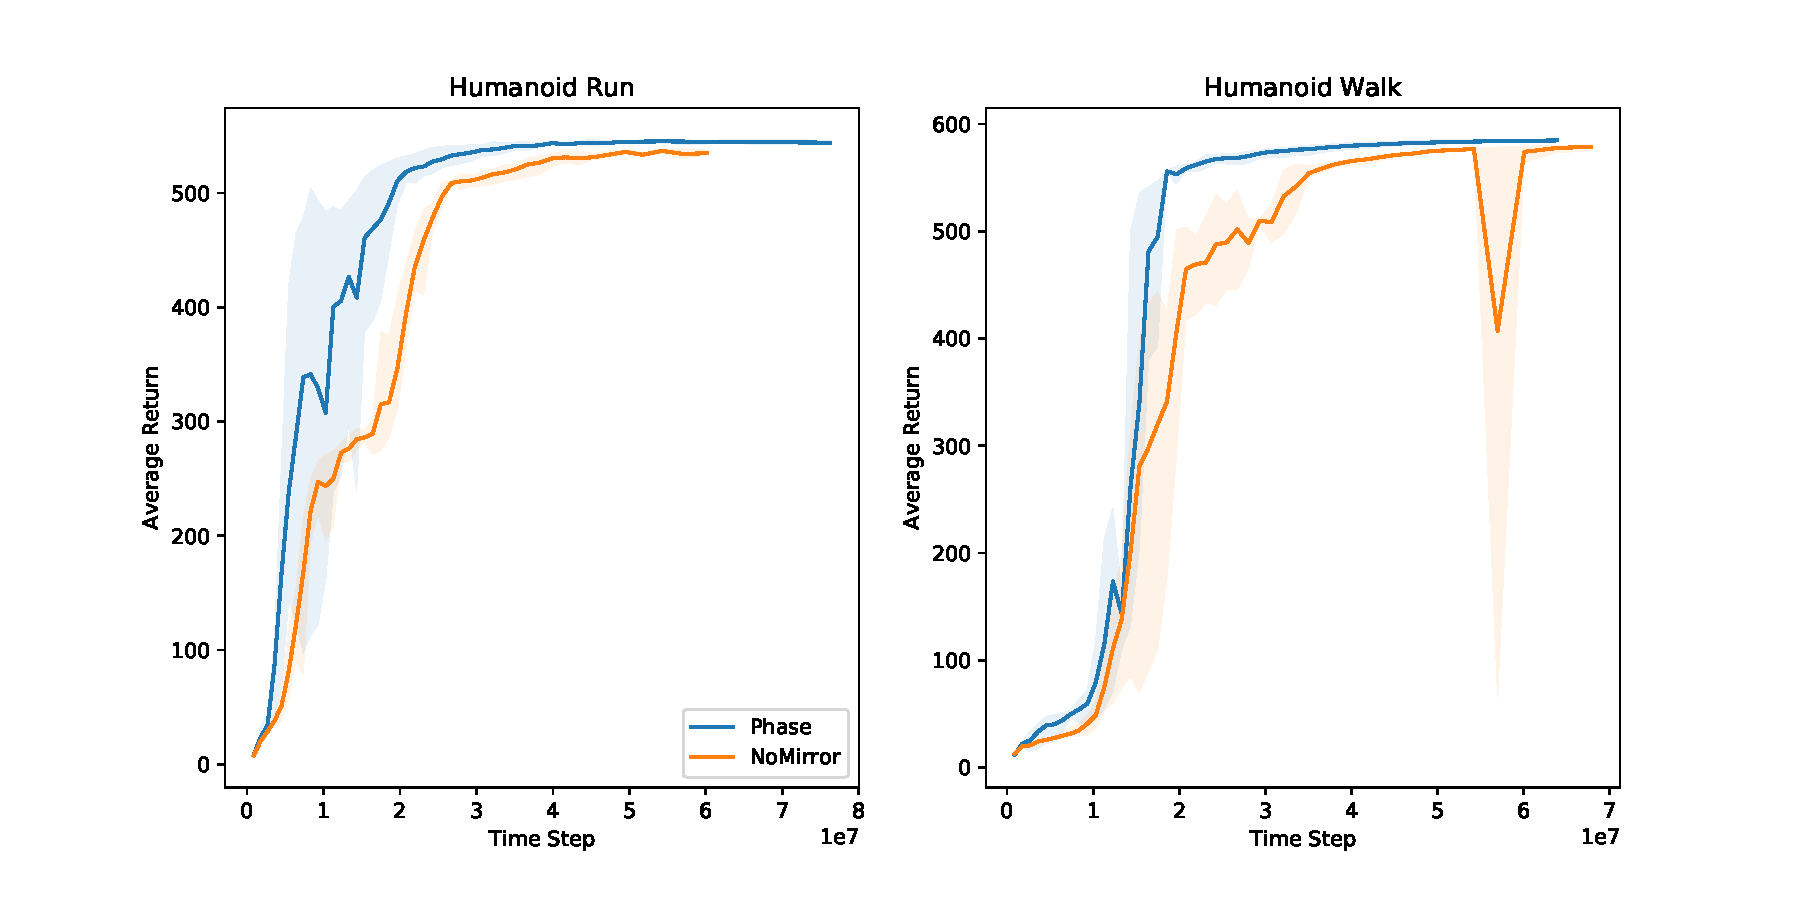
\includegraphics[width=0.9\columnwidth]{symmetry_figures/DeepMimic_curves.pdf}
  \caption{Learning curves for the original \textit{DeepMimic} environment. BASE and \textit{Phase} corresponds to the symmetry enforcement methods in \Cref{fig:learning-curves}}
  \label{fig:deepmimic-curves}
\end{figure}

\backmatter
%    7. Index
% See the makeindex package: the following page provides a quick overview
% <http://www.image.ufl.edu/help/latex/latex_indexes.shtml>


\end{document}
